% graphs.tex
% Updated January 11, 2012

\chapter{Graph Theory}\label{ch:graphs}

In \hyperref[ex:radiostations]{Example~\ref*{ex:radiostations}}, we
discussed the problem of assigning frequencies to radio stations in
the situation where stations within $200$ miles of each other must
broadcast on distinct frequencies. Clearly we would like to use the
smallest number of frequencies possible for a given layouts of
transmitters, but how can we determine what that number is?

Suppose three new homes are being built and each of them must be
provided with utility connections. The utilites in question are water,
electricity, and natural gas. Each provider needs a direct line from
their terminal to each house (the line can zig-zag all it wants, but
it must go from the terminal to the house without passing through
another provider's terminal or another house en route), and the three
providers all wish to bury their lines exactly four feet below
ground. Can they do this successfully without the lines crossing?

These are just two of many, many examples where the discrete structure
known as a \emph{graph} can serve as an enlightening mathematical
model. Graphs are perhaps the most basic and widely studied
combinatorial structure, and they are prominently featured in this
text. Many of the concepts we will study, while presented in a more
abstract mathematical sense, have their origins in applications of
graphs as models for real-world problems.

\section{Basic Notation and Terminology for Graphs}\label{s:graphs:intro}

A \textit{graph} $\bfG$ is a pair $(V,E)$ where $V$ is a set (almost
always finite) and $E$ is a set of $2$-element subsets of $V$.
Elements of $V$ are called \textit{vertices} and elements of $E$ are
called \textit{edges}.  We call $V$ the \textit{vertex set} of $\bfG$
and $E$ is the \textit{edge set}.  For convenience, it is customary to
abbreviate the edge $\{x,y\}$ as just $xy$.  Remember though that
$xy\in E$ means exactly the same as $yx\in E$.  If $x$ and $y$ are
distinct vertices from $V$, $x$ and $y$ are \textit{adjacent} when
$xy\in E$; otherwise, we say they are \textit{non-adjacent}. We say
the edge $xy$ is \emph{incident to} the vertices $x$ and $y$.

For example, we could define a graph $\GVE$ with vertex set
$V=\{a,b,c,d,e\}$ and edge set $E=\{\{a,b\},\{c,d\},\{a,d\}\}$. Notice
that no edge is incident to $e$, which is perfectly permissible based
on our definition. It is quite common to identify a graph with a
visualization in which we draw a point for each vertex and a line
connecting two vertices if they are adjacent. The graph $\bfG$ we've
just defined is shown in \autoref{fig:small_graph}. It's important to
remember that while a drawing of a graph is a helpful too, it is not
the same as the graph. We could draw $\bfG$ in any of several
different ways without changing what it is as a graph.

\begin{figure}[h]
  \centering
  \begin{overpic}{graphs-figs/small_graph}
    \put(58,100){$a$}
    \put(100,48){$b$}
    \put(-7,10){$c$}
    \put(15,50,){$d$}
    \put(70,11){$e$}
  \end{overpic}
  \caption{A graph on $5$ vertices}
  \label{fig:small_graph}
\end{figure}

As is often the case in science and mathematics, different authors use
slightly different notation and terminology for graphs.  As an
example, some use \textit{nodes} and \textit{arcs} rather than
vertices and edges.  Others refer to vertices as \textit{points} and
in this case, they often refer to \textit{lines} rather than edges.
We will try to stick to vertices and edges but confess that we may
occasionally lapse into referring to vertices as points.  Also,
following the patterns of many others, we will also say that adjacent
vertices are \textit{neighbors}.  And we will use the more or less
standard terminology that the \textit{neighborhood} of a vertex $x$ is
the set of vertices adjacent to $x$. Thus, using the graph $\bfG$ we
have depicted in \autoref{fig:small_graph}, vertices $d$ and $a$ are
neighbors, and the neighborhood of $d$ is $\{a,c\}$ while the
neighborhood of $e$ is the empty set. Also, the \textit{degree} of a
vertex $v$ in a graph $\bfG$, denoted $\deg_\bfG(v)$, is then the
number of vertices in its neighborhood, or equivalently, the number of
edges incident to it. For example, we have
$\deg_\bfG(d)=\deg_\bfG(a)=2$, $\deg_\bfG(c)=\deg_\bfG(b)=1$, and
$\deg_\bfG(e)=0$. If the graph being discussed is clear from context,
it is not uncommon to omit the subscript and simply write $\deg(v)$
for the degree of $v$.

When $\GVE$ and $\HWF$ are graphs, we say $\bfH$ is a
\textit{subgraph} of $\bfG$ when $W\subseteq V$ and $F\subseteq E$.
We say $\bfH$ is an \textit{induced} subgraph when $W\subseteq V$ and
$F=\{xy\in E: x,y\in W\}$. In other words, an induced subgraph is
defined completely by its vertex set and the original graph $\bfG$. We
say $\bfH$ is a \textit{spanning} subgraph when $W=V$. In
\autoref{fig:subgraphs}, we show a graph, a subgraph and an induced
subgraph. Neither of these subgraphs is a spanning subgraph.

\begin{figure}
\begin{center}
\includegraphics*[width=4in]{graphs-figs/subgraphs}
\caption{\label{fig:subgraphs}A Graph, a Subgraph and an Induced Subgraph}
\end{center}
\end{figure}

A graph $\GVE$ is called a \textit{complete} graph when $xy$ is an
edge in $\bfG$ for every distinct pair $x,y\in V$.  Conversely, $\bfG$
is an \textit{independent} graph if $xy\not\in E$, for every distinct
pair $x,y\in V$.  It is customary to denote a complete graph on $n$
vertices by $\bfK_n$ and an independent graph on $n$ vertices by
$\bfI_n$. In \autoref{fig:complete_graphs}, we show the complete
graphs with at most $5$ vertices.

\begin{figure}
  \centering
  \begin{overpic}[width=4in]{graphs-figs/complete_graphs}
    \put(2.5,2){$\bfK_1$}
    \put(16.5,2){$\bfK_2$}
    \put(36.5,2){$\bfK_3$}
    \put(60.5,2){$\bfK_4$}
    \put(86,2){$\bfK_5$}
  \end{overpic}
  \caption{Small complete graphs}
  \label{fig:complete_graphs}
\end{figure}

A sequence $(x_1,x_2,\dots,x_n)$ of vertices in a graph $\GVE$ is
called a \textit{walk} when $x_ix_{i+1}$ is an edge for each
$i=1,2,\dots,n-1$.  Note that the vertices in a walk need not be
distinct.  On the other hand, if the vertices are distinct, then the
sequence is called a \textit{path}, and often to emphasize where a
path starts and ends, we will say that a sequence
$(x_1,x_2,\dots,x_n)$ of distinct vertices is a path from $x_1$ to
$x_n$ in $\bfG$. Similarly, when $n\ge3$, a path $(x_1,x_2,\dots,x_n)$
of $n$ distinct vertices is called a cycle when $x_1x_n$ is also an
edge in $\bfG$.  It is customary to denote a path on $n$ vertices by
$\bfP_n$, while $\bfC_n$ denotes a cycle on $n$ vertices. The
\emph{length} of a path or a cycle is the number of edges it
contains. Therefore, the length of $\bfP_n$ is $n-1$ and the length of
$\bfC_n$ is $n$. In \autoref{fig:paths}, we show the paths of length
at most $4$, and in \autoref{fig:cycles}, we show the cycles of length
at most $5$.

\begin{figure}
  \centering
  \begin{overpic}[width=4in]{graphs-figs/paths}
    \put(8,-2){$\bfP_1$}
    \put(24,-2){$\bfP_2$}
    \put(39.5,-2){$\bfP_3$}
    \put(59.5,-2){$\bfP_4$}
    \put(85,-2){$\bfP_5$}
  \end{overpic}
  \caption{Short paths}
  \label{fig:paths}
\end{figure}
\begin{figure}
  \centering
  \begin{overpic}[width=4in]{graphs-figs/cycles}
    \put(24,1){$\bfC_3$}
    \put(47.5,1){$\bfC_4$}
    \put(73,1){$\bfC_5$}
  \end{overpic}
  \caption{Small cycles}
  \label{fig:cycles}
\end{figure}


If $\GVE$ and $\HWF$ are graphs, we say $\bfG$ is \textit{isomorphic}
to $\bfH$ and write $\bfG\cong\bfH$ when there exists a bijection
$f:V\bijection W$ so that $x$ is adjacent to $y$ in $\bfG$ if and only
if $f(x)$ is adjacent to $f(y)$ in $\bfH$.  Often writers will say
that $\bfG$ ``contains'' $\bfH$ when there is a subgraph of $\bfG$
which is isomorphic to $\bfH$.  In particular, it is customary to say
that $\bfG$ contains the cycle $\bfC_n$ (same for $\bfP_n$ and
$\bfK_n$) when $\bfG$ contains a subgraph isomorphic to $\bfC_n$. The
graphs in \autoref{fig:isomorphic} are isomorphic. An isomorphism
between these graphs is given by
\[f(a)=5,\quad f(b) = 3, \quad f(c) = 1,\quad f(d) = 6,\quad f(e)=2,\quad f(h)=4.\]
\begin{figure}
  \centering
  \begin{overpic}[width=4in]{graphs-figs/isomorphic_graphs}
    \put(6,13){$a$}
    \put(20.5,1){$b$}
    \put(36,14){$c$}
    \put(20,21){$d$}
    \put(38,2){$e$}
    \put(22.5,13){$h$}

    \put(83,13.5){$1$}
    \put(67,10){$2$}
    \put(85,2){$3$}
    \put(67.5,21.5){$4$}
    \put(53,13){$5$}
    \put(68,1){$6$}
  \end{overpic}
  \caption{A pair of isomorphic graphs}
  \label{fig:isomorphic}
\end{figure}
On the other hand, the graphs shown in \autoref{fig:nonisomorphic} are
\emph{not} isomorphic, even though they have the same number of
vertices and the same number of edges. Can you tell why?
\begin{figure}
  \centering
  \begin{overpic}[width=4in]{graphs-figs/nonisomorphic_graphs}
    \put(6,13){$a$}
    \put(20.5,1){$b$}
    \put(36,14){$c$}
    \put(20,21){$d$}
    \put(38,2){$e$}
    \put(22.5,13){$h$}

    \put(83,13.5){$1$}
    \put(73.2,10){$2$}
    \put(85,2){$3$}
    \put(67.5,21.5){$4$}
    \put(53,13){$5$}
    \put(68,1){$6$}
  \end{overpic}
  \caption{A pair of nonisomorphic graphs}
  \label{fig:nonisomorphic}
\end{figure}


 A graph $\bfG$ is \textit{connected} when there is
a path from $x$ to $y$ in $\bfG$, for every $x,y\in V$; otherwise, we
say $\bfG$ is \textit{disconnected}. The graph of
\autoref{fig:small_graph} is disconnected (a sufficient justification
for this is that there is no path from $e$ to $c$), while those in
\autoref{fig:isomorphic} are connected.

A graph is \textit{acyclic} when it does not contain any cycle on
three or more vertices.  Acyclic graphs are also called
\textit{forests}.  A connected acyclic graph is called a
\textit{tree}.  When $\GVE$ is a connected graph, a subgraph $\HWF$ of
$\bfG$ is called a \textit{spanning tree} if $\bfH$ is both a spanning
subgraph of $\bfG$ and a tree. In \autoref{fig:spantree}, we show a
graph and one of its spanning trees. We will return to the subject of
spanning trees in \autoref{ch:graphalgorithms}.
\begin{figure}
\begin{center}
\includegraphics*[width=4in]{graphs-figs/spanning_tree}
\caption{\label{fig:spantree}A Graph and a Spanning Tree}
\end{center}
\end{figure}

The following theorem is very elementary, and some authors refer to it
as the ``first theorem of graph theory''. However, this basic result
can be surprisingly useful.

\begin{theorem}
  Let $\deg_\bfG(v)$ denote the degree of vertex $v$ in graph $\GVE$. Then
  \[\sum_{v\in V}\deg_\bfG(v) = 2|E|.\eqno{(*)}\]
\end{theorem}

\begin{proof}
  We consider how many times an edge $e=vw\in E$ contributes to each
  side of (*). The $\deg_\bfG(x)$ and $\deg_\bfG(y)$ terms on the left
  hand side each count $e$ once, so $e$ is counted twice on that
  side. On the right hand side, $e$ is clearly counted
  twice. Therefore, we have the equality claimed.
\end{proof}

\begin{corollary}
  For any graph, the number of vertices of odd degree is even.
\end{corollary}

We will return to the topic of trees later, but before moving on, let
us prove one elementary proposition about trees. First, a
\textit{leaf} in a tree $\bfT$ is a vertex $v$ with $\deg_\bfT(v)=1$.

\begin{proposition}\label{prop:tree-leaves}
  Every tree on $n\geq 2$ vertices has at least two leaves.
\end{proposition}

\begin{proof}
  Our proof is by induction on $n$. For $n=2$, there is precisely one
  tree, which is isomorphic to $\bfK_2$. Both vertices in this graph
  are leaves, so the proposition holds for $n=2$. Now suppose that for
  some integer $m\geq 2$, every tree on at most $m$ vertices has at
  least two leaves and let $\bfT=(V,E)$ be a tree on $m+1$ vertices.
  Pick an edge $e\in E$ and form a new graph $\bfT'=(V',E')$ by
  deleting $e$ from $\bfT$. That is, $V'=V$ and $E'=E-\{e\}$. Now
  since $\bfT'$ does not contain a path from one endpoint of $e$ to
  its other endpoint, $\bfT'$ is not connected. However, deleting an
  edge cannot create a cycle, so $\bfT'$ is a forest. Furthermore, it
  has precisely two components, each of which is a tree with at most
  $m$ vertices. If each component has at least two vertices, then by
  induction, each has at least two leaves. In the worst case scenario,
  two of these leaves are the endpoints of $e$, so at least two of the
  vertices are leaves in $\bfT$, too. If each component of $\bfT'$ has
  only one vertex, then $\bfT\cong \bfK_2$, which has two leaves. If
  exactly one of the components has only one vertex, then it must be a
  leaf in $\bfT$. Thus, applying the inductive hypothesis to the other
  component ensures that there is a second leaf in $\bfT$.
 % First note that $\bfT$ must have a leaf, as if all vertices had
  % degree at least $2$, you could start at a vertex $v$ and walk from
  % $v$ to another vertex $v'$ and from $v'$ to another vertex and so on
  % but would eventually double back on the vertices you'd already
  % visited, since any time you visit a vertex for the first time there
  % is a way to exit the vertex to another vertex. This would create a
  % cycle, contrary to the fact that $\bfT$ is a tree. Let $v_0$ be the
  % leaf that we know must exist and let $\bfT'$ be the subgraph of
  % $\bfT$ induced by all the vertices \emph{except} $v_0$. Then $\bfT'$
  % is also a tree (removing $v_0$ cannot create a disconnected graph)
  % and has $m$ vertices, so by induction $\bfT'$ has at least two
  % leaves, $v_1$ and $v_2$. At least one of $v_1$ and $v_2$ is also a
  % leaf in $\bfT$, since $v_0$ can be adjacent to at most one of them,
  % and therefore $\bfT$ has at least two leaves.
\end{proof}

\section{Multigraphs:  Loops and Multiple Edges}\label{s:graphs:multigraphs}

Consider a graph in which the vertices represent cities and the edges
represent highways.  Certain pairs of cities are joined by an edge
while other pairs are not.  The graph may or may not be connected
(although a disconnected graph is likely to result in disgruntled
commuters).  However, certain aspects of real highway networks are not
captured by this model. First, between two nearby cities, there can
actually be several interconnecting highways, and traveling on one
of them is fundamentally different from traveling on another.  This
leads to the concept of \textit{multiple edges}, i.e., allowing for
more than one edge between two adjacent vertices.  Also, we could have
a highway which leaves a city, goes through the nearby countryside and
the returns to the same city where it originated.  This leads to the
concept of a \textit{loop}, i.e., an edge with both end points being
the same vertex.  Also, we can allow for more than one loop with the
same end point.

Accordingly, authors frequently lead off a discussion on a graph
theory topic with a sentence or two like:
\begin{enumerate}
\item In this paper, all graphs will be \textit{simple}, i.e., we will
  not allow loops or multiple edges.
\item In this paper, graphs can have loops and multiple edges.
\end{enumerate}
The terminology is far from standard, but in this text, a graph will
always be a \textit{simple} graph, i.e., no loops or multiple edges.
When we want to allow for loops and multiple edges, we will use the
term \textit{multigraph}.  This begs the question of what we would
call a graph if it is allowed to have loops but not multiple edges, or
if multiple edges are allowed but not loops.  If we \textit{really}
needed to talk about such graphs, then the English language comes to
our rescue, and we just state the restriction explicitly!

\section{Eulerian and Hamiltonian Graphs}\label{s:graphs:eulerham}

Graph theory is an area of mathematics that has found many
applications in a variety of disciplines. Throughout this text, we
will encounter a number of them. However, graph theory traces its
origins to a problem in K\"onigsberg, Prussia (now Kaliningrad,
Russia) nearly three centuries ago. The river Pregel passes through
the city, and there are two large islands in the middle of the
channel. These islands were connected to the mainland by seven bridges
as indicated in \autoref{fig:bridges}. It is said that the citizens of
K\"onigsberg often wondered if it was possible for one to leave his
home, walk through the city in such a way that he crossed each bridge
precisely one time, and end up at home again. Leonhard Euler settled
this problem in 1736 by using graph theory in the form of
\autoref{thm:eulerian}.

\begin{figure}
  \centering
  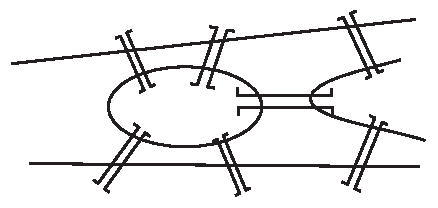
\includegraphics{graphs-figs/konigsberg_bridges}
  \caption{\label{fig:bridges}The bridges of K\"onigsberg}
\end{figure}

A graph $\bfG$ is \textit{eulerian} if there is a sequence
$(x_0,x_1,x_2,\dots,x_t)$ of vertices from $\bfG$, with repetition
allowed, so that
\begin{enumerate}
\label{def:eulerian-circuit}
\item $x_0=x_t$;
\item for every $i=0,1,\dots t-1$, $x_ix_{i+1}$ is an edge of $\bfG$;
\item for every edge $e\in E$, there is a unique
  integer $i$ with $0\le i<t$ for which $e=x_ix_{i+1}$.
\end{enumerate}
When $\bfG$ is eulerian, a sequence satisfying these three conditions
is called an \textit{eulerian circuit}. A sequence of vertices
$(x_0,x_1,\dots,x_t)$ is called a \textit{circuit} when it satisfies
only the first two of these conditions.  Note that a sequence
consisting of a single vertex is a circuit. The following elementary
theorem completely characterizes eulerian graphs.  It comes with an
algorithmic proof, one that is easily implemented.

\begin{theorem}\label{thm:eulerian}
  A graph $\bfG$ is eulerian if and only if it is connected and 
  every vertex has even degree.
\end{theorem}

\begin{proof}
  Clearly, an eulerian graph must be connected.  Also, if $(x_0,x_1,\dots,x_t)$
  is an eulerian circuit in $\bfG$, then for each $i=0,1,\dots,t-1$,
  we can view the edge $x_ix_{i+1}$ as exiting $x_i$ and entering $x_{i+1}$.
  The degree of every vertex must be even, since for each vertex $x$, the
  number of edges exiting $x$ equals the number of edges entering $x$.
  Furthermore, each edge incident with $x$ either exits from $x$ or enters~$x$.

  We now describe a deterministic process that will either (a)~find
  an eulerian circuit, (b) show that the graph is disconnected, or
  (c)~find a vertex of odd degree.
  The description is simplified by assuming that the vertices in
  $\bfG$ have been labelled with the positive integers $1,2,\dots,n$, where
  $n$ is the number of vertices in $\bfG$.  Furthermore, we take $x_0=1$.

  We launch our algorithm with a trivial circuit $C$ consisting of
  just the vertex $x_0=(1)$.  Thereafter suppose that we have a partial
  circuit $C$ defined by a sequence $(x_0, x_1,\dots,x_t)$ with
  $x_0=x_t=1$. The edges
  of the form $x_ix_{i+1}$ have been \textit{traversed}, while the
  remaining edges in $\bfG$ (if any) have not.  If the third condition
  for an euler circuit is satisfied, we are done, so we assume it does
  not hold.

  We then choose the least integer $i$ for which there is an edge
  incident with $x_i$ that has not already been traversed.  If there
  is no such integer, since there are edges that have not yet been
  traversed, then we have discovered that the graph is disconnected.
  So we may assume that the integer $i$ exists.  Set $u_0=x_i$.  We
  define a sequence $(u_0,u_1,\dots,u_s)$ recursively.  If $j\ge 0$, set
  \[
   N_j=\{y: u_jy\text{ is an edge in $\bfG$ and has not yet been traversed.}\}
 \] 
  If  $N_j\neq\emptyset$, we take $u_{j+1}$ as the least positive integer
  in $N_j$. If $N_j=\emptyset$, then $j\ge1$ and we take $s=j$ and halt
  this subroutine.
  
  When the subroutine halts, we consider two cases.  If $u_0\neq u_s$,
  then $u_0$ and $u_s$ are vertices of odd degree in  $\bfG$.  So we
  are left to consider the case where $u_0=u_s=x_i$.  In this case,
  we simply expand our original sequence $(x_0,x_1,\dots,x_t)$ by
  replacing the integer $x_i$ by the sequence $(u_0,u_1,\dots,u_s)$.
\end{proof}

As an example, consider the graph $\bfG$ shown in \autoref{fig:graphs:eulerexample}.
Evidently, this graph is connected and all vertices have even degree.
Here is the sequence of circuits starting with the trivial circuit $C$
consisting only of the vertex~$1$.
\begin{align*}
C &=(1)\\
  &=(1,2,4,3,1)\quad \text{start next from $2$}\\ 
  &=(1,2,5,8,2,4,3,1)\quad\text{start next from $4$}\\
  &=(1,2,5,8,2,4,6,7,4,9,6,10,4,3,1)\quad\text{start next from $7$}\\
  &=(1,2,5,8,2,4,6,7,9,11,7,4,9,6,10,4,3,1)\quad\text{Done!!}
\end{align*}	
  
\begin{figure}
  \centering
  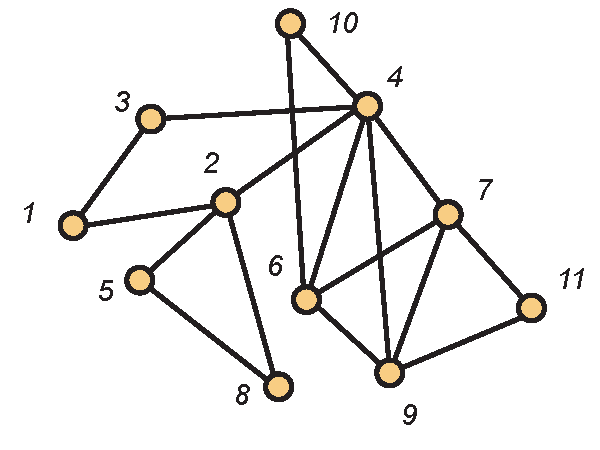
\includegraphics[width=2.5in]{graphs-figs/eulerian_graph}

  \caption{An Eulerian Graph}
  \label{fig:graphs:eulerexample}
\end{figure}
You should note that \autoref{thm:eulerian} holds for loopless graphs
in which multiple edges are allowed.  Euler used his theorem to show
that the multigraph of K\"onigsberg shown in
\autoref{fig:bridges-graph}, in which each land mass is a vertex and
each bridge is an edge, is \textit{not} eulerian, and thus the
citizens could not find the route they desired. (Note that in
\autoref{fig:bridges-graph} there are multiple edges between the same
pair of vertices.)

\begin{figure}[h]
  \centering
  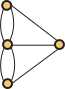
\includegraphics{graphs-figs/konigsberg_graph}
  \caption{The multigraph of K\"onigsberg's bridges}
  \label{fig:bridges-graph}
\end{figure}

A graph $\GVE$ is said to be \textit{hamiltonian} if there exists a
sequence $(x_1,x_2,\dots,x_n)$ so that
\begin{enumerate}
\item every vertex of $\bfG$ appears exactly once in the sequence;
\item $x_1x_n$ is an edge of $\bfG$; and
\item for each $i=1,2,\dots,n-1$, $x_ix_{i+1}$ is an edge in $\bfG$.
\end{enumerate}

The first graph shown in \autoref{fig:eulham} both eulerian and
hamiltonian.  The second is hamiltonian but not eulerian.
\begin{figure}
\begin{center}
\includegraphics*[width=3.55in]{graphs-figs/eulerian_hamiltonian_crop}
\caption{\label{fig:eulham}Eulerian and Hamiltonian Graphs}
\end{center}
\end{figure}

In \autoref{fig:petersen}, we show a famous graph known
as the Petersen graph. It is not hamiltonian.
% Might we want to include the proof of this?
\begin{figure}
\begin{center}
\includegraphics*[width=0.56\textwidth]{graphs-figs/petersen_graph}
\caption{\label{fig:petersen}The Petersen Graph}
\end{center}
\end{figure}

Unlike the situation with eulerian circuits, there is no
known method for quickly determining whether a graph is
hamiltonian.  However, there are a number of interesting
conditions which are sufficient.  Here is one quite well
known example, due to Dirac.

\begin{theorem}\label{thm:graphs:dirac}
If $\bfG$ is a graph on $n$ vertices and each vertex
in $\bfG$ has at least $\lceil \frac{n}{2}\rceil$ neighbors,
then $\bfG$ is hamiltonian.
\end{theorem}

\begin{proof}
Suppose the theorem fails and let $n$ be the least positive
integer for which there exists a graph $\bfG$ on $n$ vertices
so that each vertex in $\bfG$ has at least $\lceil n/2\rceil$
neighbors, yet there is no hamiltonian cycle in $\bfG$. Clearly,
$n\ge4$.

Now let $t$ be the largest integer for which $\bfG$ has
a path $P=(x_1,x_2,\dots,x_t)$ on $t$ vertices.  Clearly all
neighbors of both $x_1$ and $x_t$ appear on this path.  By
the pigeon hole principle, there is some integer $i$ with
$1\le i<t$ so that $x_1x_{i+1}$ and $x_{i}x_t$ are edges
in $\bfG$.  However, this implies that
\[
C=(x_1,x_2,x_3,\dots,x_i,x_t,x_{t-1},x_{t-2},\dots,x_{i+1})
\]
is a cycle of length $t$ in $\bfG$. In turn, this 
requires $\lceil n/2\rceil < t<n$.  But if $y$ is any vertex
not on the cycle, then $y$ must have a neighbor on $C$, which
implies that $\bfG$ has a path on $t+1$ vertices.  The contradiction
completes the proof.
\end{proof}

\section{Graph Coloring}\label{s:graphs:color}

Let's return now to the subject of
\hyperref[ex:radiostations]{Example~\ref*{ex:radiostations}},
assigning frequencies to radio stations so that they don't
interfere. The first thing that we will need to do is to turn the map
of radio stations into a suitable graph, which should be pretty
natural at this juncture. We define a graph $\GVE$ in which $V$ is the
set of radio stations and $xy\in E$ if and only if radio station $x$
and radio station $y$ are within $200$ miles of each other. With this
as our model, then we need to assign different frequencies to two
stations if their corresponding vertices are joined by an edge. This
leads us to our next topic, coloring graphs.

When $\GVE$ is a graph and $C$ is a set of elements called
\textit{colors}, a \textit{proper coloring} of $\bfG$ is a function
$\phi:V\to C$ such that if $\phi(x)\neq \phi(y)$ whenever $xy$ is an
edge in $\bfG$.  The least $t$ for which $\bfG$ has a proper coloring
using a set $C$ of $t$ colors is called the \textit{chromatic number}
of $\bfG$ and is denoted $\chi(\bfG)$.  In \autoref{fig:graphs:chi4},
we show a proper coloring of a graph using $5$ colors. Now we can see
that our radio frequency assignment problem is the much-studied
question of finding the chromatic number of an appropriate graph.
\begin{figure}[h]
\begin{center}
\includegraphics*[scale=0.63]{graphs-figs/chi4}
\caption{\label{fig:graphs:chi4}A proper coloring using $5$ colors}
\end{center}
\end{figure}

\begin{discussion}
  Everyone agrees that the graph $\bfG$ in \autoref{fig:graphs:chi4}
  has chromatic number at most $5$. However, there's a bit of debate
  going on about if $\chi(\bfG)=5$. Bob figures the authors would not
  have used five colors if they didn't need to. Carlos says he's glad
  they're having the discussion, since all having a proper coloring
  does is provide them with an upper bound on $\chi(\bfG)$. Bob sees
  that the graph has a vertex of degree $5$ and claims that must mean
  $\chi(\bfG)=5$. Alice groans and draws a graph with $101$ vertices,
  one of which has degree $100$, but with chromatic number $2$. Bob is
  shocked, but agrees with her. Xing wonders if the fact that the
  graph does not contain a $\bfK_3$ has any bearing on the chromatic
  number. Dave's in a hurry to get to the gym, but on his way out the
  door he says they can get a proper $4$-coloring pretty easily, so
  $\chi(\bfG)\leq 4$. The rest decide it's time to keep reading.
 \begin{itemize}
  \item What graph did Alice draw that shocked Bob?
  \item What changes did Dave make to the coloring in
    \autoref{fig:graphs:chi4} to get a proper coloring using four
    colors?
  \end{itemize}
\end{discussion}

\subsection{Bipartite Graphs}

A graph $\GVE$ with $\chi(\bfG)\le 2$ is called a $2$-\textit{colorable} graph. 
Recognizing $2$-colorable graphs is easy.

\begin{theorem}\label{thm:graphs:bipartite}
  A graph is $2$-colorable if and only if it does not contain an odd
  cycle.
\end{theorem}

\begin{proof}
  Clearly a graph containing an odd cycle cannot be $2$-colorable.
  For the converse, let $\bfG$ be a graph which does not contain
  an odd cycle.   For each component $C$ of $\bfG$, we choose
  an arbitrary vertex $r_C$ from $C$ and color all such vertices
  with color $1$.  Then for each component $C$ and each vertex
  $y\in C$ with $y\neq r_C$, let $P=(r_C=x_1,x_2,\dots,x_t=y)$ be
  a shortest path from $r_C$ to $y$.  Assign $y$ color $1$ if
  $t$ is odd and color~$2$ if $t$ is even.  It is easy to see that
  this determines a $2$-coloring of $\bfG$.
\end{proof}

A graph $\bfG$ is called a bipartite graph when there is
a partition of the vertex $V$ into two sets $A$ and $B$ 
so that the subgraphs induced by $A$ and $B$ are independent graphs, 
i.e., no edge of $\bfG$ has both of its endpoints in $A$ or in $B$. 
Evidently, bipartite graphs are $2$-colorable.  On the other hand,
when a $2$-colorable graph is disconnected, there is more than
one way to define a suitable partition of the vertex set into
two independent sets.

Bipartite graphs are commonly used as models when there are two
distinct types of objects being modeled and connections are only
allowed between two objects of different types.  For example,
on one side, list candidates who attend a career fair and on the
other side list the available positions.  The edges might naturally
correspond to candidate/position pairs which link a person to
a responsibility they are capable of handling.

As a second example, a
bipartite graph could be used to visualize the languages spoken by a
group of students. The vertices on one side would be the students with the
languages listed on the other side.  We would then have an edge $xy$ when
student $x$ spoke language $y$.
A concrete example of this graph for our favorite group of students is
shown in \autoref{fig:graphs:languages}, although Alice isn't so
certain there should be an edge connecting Dave and English.

\begin{figure}[b]
  \centering
  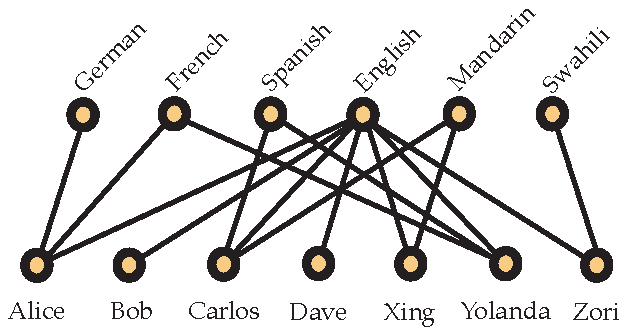
\includegraphics[scale=0.63]{graphs-figs/languages}
  \caption{A bipartite graph}
  \label{fig:graphs:languages}
\end{figure}

One special class of bipartite graphs that bears mention is the class
of \emph{complete bipartite graphs}. The complete bipartite graph
$\bfK_{m,n}$ has vertex set $V=V_1\cup V_2$ with $|V_1|=m$ and
$|V_2|=n$. It has an edge $xy$ if and only if $x\in V_1$ and $y\in
V_2$. The complete bipartite graph $\bfK_{3,3}$ is shown in \autoref{fig:graphs:k33}.

\begin{figure}[h]
  \centering
  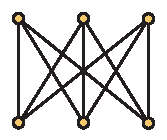
\includegraphics{graphs-figs/k33_rotated}
  \caption{The complete bipartite graph $\bfK_{3,3}$}
  \label{fig:graphs:k33}
\end{figure}

\subsection{Cliques and Chromatic Number}

A \textit{clique} in a graph $\GVE$ is a set $K\subseteq V$ such that
the subgraph induced by $K$ is isomorphic to the complete graph
$\bfK_{|K|}$. Equivalently, we can say that every pair of vertices in
$K$ are adjacent. The \textit{maximum clique size} or \textit{clique
  number} of a graph $\bfG$, denoted $\omega(\bfG)$, is the largest
$t$ for which there exists a clique $K$ with $|K|=t$.  For example,
the graph in \autoref{fig:graphs:eulerexample} has clique number $4$
while the graph in \autoref{fig:graphs:chi4} has maximum clique
size~$2$.

For every graph $\bfG$, it is obvious that $\chi(\bfG)\ge
\omega(\bfG)$.  On the other hand, the inequality may be far from
tight. Before proving showing how bad it can be, we need to introduce
a more general version of the
\hyperref[prop:pigeon]{Pigeon Hole Principle
  (Proposition~\ref*{prop:pigeon})}. Consider a function $f\colon X\to
Y$ with $|X| = 2|Y|+1$. Since $|X|>|Y|$, the Pigeon Hole Principle
as stated in \autoref{ch:basics} only tells us that there are distinct
$x,x'\in X$ with $f(x)=f(x')$. However, we can say more here. Suppose
that each element of $Y$ has at most two elements of $X$ mapped to
it. Then adding up the number of elements of $X$ based on how many are
mapped to each element of $Y$ would only allow $X$ to have (at most)
$2|Y|$ elements. Thus, there must be $y\in Y$ so that there are three
distinct elements $x,x',x''\in X$ with $f(x)=f(x')=f(x'')=y$. This
argument generalizes to give the following version of the Pigeon Hole
Principle:

\begin{proposition}\label{prop:graphs:pigeon-general}
  If $f\colon X\to Y$ is a function and $|X|\geq (m-1)|Y|+1$, then
  there exists an element $y\in Y$ and distinct elements
  $x_1,\dots,x_m \in X$ so that $f(x_i)=y$ for $i=1,\dots,m$.
\end{proposition}

We are now prepared to present the following proposition showing that
clique number and chromatic number need not be close at all.

\begin{proposition}\label{prop:triangle-free}
  For every $t\ge3$, there exists a graph $\bfG_t$ so that
  $\chi(\bfG_t)=t$ and $\omega(\bfG_t)=2$
\end{proposition}

\begin{proof}[Proof (J. Kelly and L. Kelly)]
  We proceed by induction on $t$. For $t=3$, we take $\bfG_3$ to be
  the cycle $\bfC_5$ on five vertices.  Now assume that for some
  $t\ge3$, we have determined the graph $\bfG_t$.  Suppose that
  $\bfG_t$ has $n_t$ vertices.  Label the vertices of $\bfG_t$ as
  $x_1,x_2,\dots,x_{n_t}$.  Construct $\bfG_{t+1}$ as follows.  Begin
  with an independent set $I$ of cardinality $t(n_t-1)+1$.  For every
  subset $S$ of $I$ with $|S|=n_t$, label the elements of $S$ as
  $y_1,y_2,\dots,y_{n_t}$.  For this particular $n_t$-element subset
  attach a copy of $\bfG_t$ with $y_i$ adjacent to $x_i$ for
  $i=1,2,\dots,n_t$.  Vertices in copies of $\bfG_t$ for distinct
  $n_t$-element subsets of $I$ are nonadjacent, and a vertex in $I$
  has at most one neighbor in a particular copy of $\bfG_t$.

  To see that $\omega(\bfG_{t+1})=2$, it will suffice to argue that
  $\bfG_{t+1}$ contains no triangle ($\bfK_3$).  Since $\bfG_t$ is
  triangle-free, any triangle in $\bfG_{t+1}$ must contain a vertex of
  $I$. Since none of the vertices of $I$ are adjacent, any triangle in
  $\bfG_{t+1}$ contains only one point of $I$. Since each vertex of
  $I$ is adjacent to at most one vertex of any fixed copy of $\bfG_t$,
  if $y\in I$ is part of a triangle, the other two vertices must come
  from distinct copies of $\bfG_t$. However, vertices in different
  copies of $\bfG_t$ are not adjacent, so
  $\omega(\bfG_{t+1})=2$. Notice that $\chi(\bfG_{t+1})\ge t$ since
  $\bfG_{t+1}$ contains $\bfG_t$.  On the other hand,
  $\chi(\bfG_{t+1})\le t+1$ since we may use $t$ colors on the copies
  of $\bfG_t$ and a new color on the independent set $I$.  To see that
  $\chi(\bfG_{t+1})=t+1$, observe that if we use only $t$ colors, then
  by the generalized Pigeon Hole Principle, there is an $n_t$-element
  subset of $I$ in which all vertices have the same color.  Then this
  color cannot be used in the copy of $\bfG_t$ which is attached to
  that $n_t$-element subset.
\end{proof}

Here is another argument for the same result.

\begin{proof}[Proof (J. Mycielski)]
  We again start with $\bfG_3$ as the cycle $\bfC_5$.  As before we
  assume that we have constructed for some $t\ge3$ a graph $\bfG_t$
  with $\omega(\bfG_t)=2$ and $\chi(\bfG_t) = t$.  Again, label the
  vertices of $\bfG_t$ as $x_1,x_2,\dots,x_{n_t}$.  To construct
  $\bfG_{t+1}$, we now start with an independent set $I$, but now $I$
  has only $n_t$ points, which we label as $y_1,y_2,\dots,y_{n_t}$.  We
  then add a copy of $\bfG_t$ with $y_i$ adjacent to $x_j$ if and only
  if $x_i$ is adjacent to $x_j$.  Finally, attach a new vertex $z$
  adjacent to all vertices in $I$.

  Clearly, $\omega(\bfG_{t+1})=2$.  Also,
  $\chi(\bfG_{t+1})\ge t$, since it contains $\bfG_t$ as a subgraph.
  Furthermore,
  $\chi(\bfG_{t+1})\leq t+1$, since we can color $\bfG_t$ with colors
  from $\{1,2,\dots,t\}$, use color $t+1$ on the independent set $I$,
  and then assign color~$1$ to the new vertex $z$. We claim that in fact
  $\chi(\bfG_{t+1})=t+1$. Suppose not. Then we must have
  $\chi(\bfG_{t+1})=t$.  Let $\phi$ be a proper
  coloring of $\bfG_{t+1}$.  Without loss of generality, $\phi$ uses
  the colors in $\{1,2,\dots,t\}$ and $\phi$ assigns color~$t$ to $z$.
  Then consider the nonempty set $S$ of vertices in the copy of
  $\bfG_t$ to which $\phi$ assigns color $t$.  For each $x_i$ in $S$,
  change the color on $x_i$ so that it matches the color assigned to
  $y_i$ by $\phi$, which cannot be $t$, as $z$ is colored $t$.  What
  results is a proper coloring of the copy of $\bfG_t$ with only $t-1$
  colors since $x_i$ and $y_i$ are adjacent to the same vertices of
  the copy of $\bfG_t$.  The contradiction shows that
  $\chi(\bfG_{t+1})=t+1$, as claimed.
\end{proof}

Since a $3$-clique looks like a triangle,
\hyperref[prop:triangle-free]{Proposition~\ref*{prop:triangle-free}}
is often stated as ``There exist triangle-free graphs with large
chromatic number.'' As an illustration of the construction in the
proof of Mycielski, we again refer to \autoref{fig:graphs:chi4}.  The
graph shown is $\bfG_4$. We will return to the topic of graphs with
large chromatic number in \autoref{s:probmeth:girth} where we show
that are there graphs with large chromatic number which lack not only
cliques of more than two vertices but also \emph{cycles} of less than
$g$ vertices for \emph{any} value of $g$. In other words, there is a
graph $\bfG$ with $\chi(\bfG)=10^6$ but no cycle with fewer than
$10^{10}$ vertices!

\subsection{Can We Determine Chromatic Number?}

Suppose you are given a graph $\bfG$. It's starting to look like it is
not easy to find an algorithm that answers the question ``Is
$\chi(\bfG)\leq t$?'' It's easy to verify a certificate (a proper
coloring using at most $t$ colors), but how could you even find a
proper coloring, not to mention one with the fewest number of colors?
Similarly for the question ``Is $\omega(\bfG)\geq k$?'', it is easy to
verify a certificate. However, finding a maximum clique appears to be
a very hard problem. Of course, since the gap between $\chi(\bfG)$ and
$\omega(\bfG)$ can be arbitrarily large, being able to find one value
would not (generally) help in finding the value of the other. No
polynomial-time algorithm is known for either of these problems, and
many believe that no such algorithm exists. In this subsection, we
look at one approach to finding chromatic number and see a case where
it does work efficiently.

A very na\"ive algorithmic way to approach graph coloring is the First
Fit, or ``greedy'', algorithm. For this algorithm, fix an ordering of
the vertex set $V=\{v_1,v_2,\dots v_n\}$. We define the coloring
function $\phi$ one vertex at a time in increasing order of
subscript. We begin with $\phi(v_1)=1$ and then we define
$\phi(v_{i+1})$ (assuming vertices $v_1,v_2,\dots,v_i$ have been
colored) to be the least positive integer color that has not already
been used on any of its neighbors in the set $\{v_1,\dots v_i\}$.

\begin{figure}
  \centering
  \begin{picture}(0,0)
    \put(0,76){\raisebox{0mm}[0mm][0mm]{\makebox[0mm]{$v_1$}}}%
    \put(0,52){\raisebox{0mm}[0mm][0mm]{\makebox[0mm]{$v_3$}}}%
    \put(0,29){\raisebox{0mm}[0mm][0mm]{\makebox[0mm]{$v_5$}}}%
    \put(0,7){\raisebox{0mm}[0mm][0mm]{\makebox[0mm]{$v_7$}}}%
    \put(65,76){\raisebox{0mm}[0mm][0mm]{\makebox[0mm]{$v_2$}}}%
    \put(65,52){\raisebox{0mm}[0mm][0mm]{\makebox[0mm]{$v_4$}}}%
    \put(65,29){\raisebox{0mm}[0mm][0mm]{\makebox[0mm]{$v_6$}}}%
    \put(65,7){\raisebox{0mm}[0mm][0mm]{\makebox[0mm]{$v_8$}}}%
    \put(113,76){\raisebox{0mm}[0mm][0mm]{\makebox[0mm]{$v_1$}}}%
    \put(113,52){\raisebox{0mm}[0mm][0mm]{\makebox[0mm]{$v_2$}}}%
    \put(113,29){\raisebox{0mm}[0mm][0mm]{\makebox[0mm]{$v_3$}}}%
    \put(113,7){\raisebox{0mm}[0mm][0mm]{\makebox[0mm]{$v_4$}}}%
    \put(178,76){\raisebox{0mm}[0mm][0mm]{\makebox[0mm]{$v_5$}}}%
    \put(178,52){\raisebox{0mm}[0mm][0mm]{\makebox[0mm]{$v_6$}}}%
    \put(178,29){\raisebox{0mm}[0mm][0mm]{\makebox[0mm]{$v_7$}}}%
    \put(178,7){\raisebox{0mm}[0mm][0mm]{\makebox[0mm]{$v_8$}}}%
  \end{picture}
  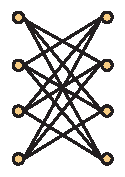
\includegraphics{graphs-figs/k44-M_crop}\hspace{.75in}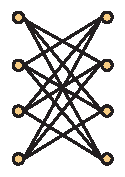
\includegraphics{graphs-figs/k44-M_crop}
  \caption{Two orderings of the vertices of a bipartite graph.}
  \label{fig:k44minus}
\end{figure}
\autoref{fig:k44minus} shows two different orderings of the same
graph. \hyperref[ex:graphs:first-fit-color]{Exercise~\ref*{ex:graphs:first-fit-color}}
demonstrates that the ordering of $V$ is vital to the ability of the
First Fit algorithm to color $\bfG$ using $\chi(\bfG)$ colors. In
general, finding an optimal ordering is just as difficult as coloring
$\bfG$. Thus, this very simple algorithm does not work well in
general. However, for some classes of graphs, there is a ``natural''
ordering that leads to optimal performance of First Fit. Here is one
such example---one that we will study again in the next chapter in a
different context.

Given an indexed family of sets $\cgF=\{S_\alpha:\alpha\in V\}$, we
associate with $\cgF$ a graph $\bfG$ defined as follows.  The vertex
set of $\bfG$ is the set $V$ and vertices $x$ and $y$ in $V$ are
adjacent in $\bfG$ if and only if $S_x\cap S_y \neq\emptyset$.  We
call $\bfG$ an \textit{intersection graph}.  It is easy to see that
every graph is an intersection graph (\emph{why?}), so it makes sense
to restrict the sets which belong to $\cgF$.  For example, we call
$\bfG$ an \textit{interval graph} if it is the intersection graph of a
family of closed intervals of the real line $\reals$. For example, in
\autoref{fig:graphs:interval-graph}, we show a collection of six
intervals of the real line on the left. On the right, we show the
corresponding interval graph having an edge between vertices $x$ and
$y$ if and only if intervals $x$ and $y$ overlap.

\begin{figure}
  \centering
  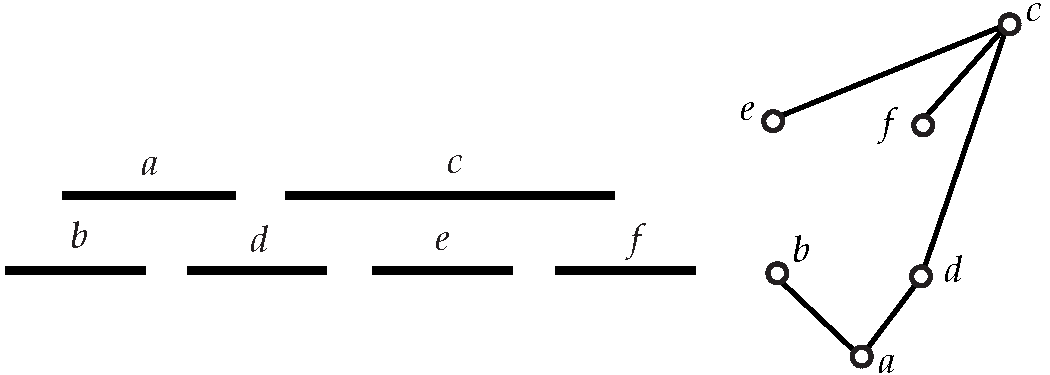
\includegraphics[scale=0.5]{graphs-figs/interval-graph}
  \caption{A collection of intervals and its interval graph}
  \label{fig:graphs:interval-graph}
\end{figure}

\begin{theorem}
  \label{thm:intgraphcol}If $\GVE$ is an interval graph, then
  $\chi(\bfG)=\omega(\bfG)$.
\end{theorem}

\begin{proof}
  For each $v\in V$, let $I(v)=[a_v,b_v]$ be a closed interval of the
  real line so that $uv$ is an edge in $\bfG$ if and only if $I(u)\cap
  I(v)\neq\emptyset$. Order the vertex set $V$ as $\{v_1,v_2,\dots
  v_n\}$ such that $a_1\leq a_2\leq \cdots \leq a_n$. (Ties may be
  broken arbitrarily.) Apply the First Fit coloring algorithm to
  $\bfG$ with this ordering on $V$. Now when the First Fit coloring
  algorithm colors $v_i$, all of its neighbors have left end point at
  most $a_i$. Since they are neighbors of $v_i$, however, we know that
  their right endpoints are all at least $a_i$. Thus, $v_i$ and its
  previously-colored neighbors form a clique. Hence, $v_i$ is adjacent
  to at most $\omega(\bfG)-1$ other vertices that have already been
  colored, so when the algorithm colors $v_i$, there will be a color
  from $\{1,2,\dots,\omega(\bfG)\}$ not already in use on its
  neighbors.  The algorithm will assign $v_i$ the smallest such
  color. Thus, we never need to use more than $\omega(\bfG)$ colors,
  so $\chi(\bfG)=\omega(\bfG)$.
\end{proof}

A graph $\bfG$ is said to be \emph{perfect} if
$\chi(\bfH)=\omega(\bfH)$ for every induced subgraph $\bfH$. Since an
induced subgraph of an interval graph is an interval graph,
\autoref{thm:intgraphcol} shows interval graphs are perfect. The study
of perfect graphs originated in connection with the theory of
communications networks and has proved to be a major area of research
in graph theory for many years now.

\section{Planar Graphs}\label{s:graphs:planar}

Let's return to the problem of providing lines for water, electricity,
and natural gas to three homes which we discussed in the introduction
to this chapter. How can we model this problem using a graph? The best
way is to have a vertex for each utility and a vertex for each of the
three homes. Then what we're asking is if we can draw the graph that
has an edge from each utility to each home so that none of the edges
cross. This graph is shown in \autoref{fig:graphs:utils}. You should
recognize it as the complete bipartite graph $\bfK_{3,3}$ we
introduced earlier in the chapter.
\begin{figure}
  \centering
  \begin{overpic}{graphs-figs/k33}
    \put(-25,92){\small Water}
    \put(-43,50){\small Electricity}
    \put(-53,5){\small Natural gas}
    \put(92,92){\small Home 1}
    \put(92,50){\small Home 2}
    \put(92,5){\small Home 3}
  \end{overpic}
  \caption{A graph of connecting homes to utilities}
  \label{fig:graphs:utils}
\end{figure}

While this example of utility lines might seem a bit contrived, since
there's really no good reason that the providers can't bury their
lines at different depths, the question of whether a graph can be
drawn in the plane such that edges intersect only at vertices is a
long-studied question in mathematics that does have useful
applications. One area where it arises is in the design of microchips
and circuit boards. In those contexts, the material is so thin that
the option of placing connections at different depths either does not
exist or is severely restricted. There is much deep mathematics that
underlies this area, and this section is intended to introduce a few
of the key concepts.

By a \textit{drawing} of a graph, we mean a way of associating its
vertices with points in the Cartesian plane $\reals^2$ and its edges
with simple polygonal arcs whose endpoints are the points associated
to the vertices that are the endpoints of the edge. You can think of a
polygonal arc as just a finite sequence of line segments such that the
endpoint of one line segment is the starting point of the next line
segment, and a simple polygonal arc is one that does not cross
itself. (Our choice of polygonal arcs rather than arbitrary curves
actually doesn't cause an impediment, since by taking very, very, very
short line segments we can approximate any curve.) A \textit{planar
  drawing} of a graph is one in which the polygonal arcs corresponding
to two edges intersect only at a point corresponding to a vertex to
which they are both incident. A graph is \textit{planar} if it has a
planar drawing. A \textit{face} of a planar drawing of a graph is a
region bounded by edges and vertices and not containing any other
vertices or edges.

\autoref{fig:planar} shows a planar drawing of a graph with $6$
vertices and $9$ edges. Notice how one of the edges is drawn as a true
polygonal arc rather than a straight line segment. This drawing
determines $5$ regions, since we also count the unbounded region that
surrounds the drawing.
\begin{figure}[b]
  \centering
  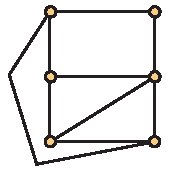
\includegraphics{graphs-figs/planar_graph}
  \caption{A planar drawing of a graph}
  \label{fig:planar}
\end{figure}
\autoref{fig:k4-planar} shows a planar drawing of the complete graph
$\bfK_4$. There are $4$ vertices, $6$ edges, and $4$ faces in the
drawing.
\begin{figure}[ht]
  \centering
  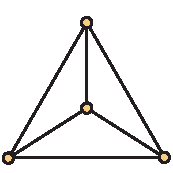
\includegraphics{graphs-figs/k4_planar}
  \caption{A planar drawing of $\bfK_4$}
  \label{fig:k4-planar}
\end{figure}
What happens if we compute the number of vertices minus the number of
edges plus the number of faces for these drawings? We have
\begin{align*}
  6-9+5 &= 2\\
  4-6+4 &=2
\end{align*}
While it might seem like a coincidence that this computation results
in $2$ for these planar drawings, there's a more general principle at
work here, and in fact it holds for \emph{any} planar drawing of
\emph{any} planar graph.

\begin{theorem}[Euler]
  Let $\bfG$ be a connected planar graph with $n$ vertices and $m$
  edges. Every planar drawing of $\bfG$ has $f$ faces, where $f$
  satisfies
  \[n-m+f=2.\]
\end{theorem}

The number $2$ here actually results from a fundamental property of
the plane, and there are a corresponding theorems for other
surfaces. However, we only need the result as stated above.

\begin{proof}
  Our proof is by induction on the number $m$ of edges. If $m=0$, then
  since $\bfG$ is connected, our graph has a single vertex, and so
  there is one face. Thus $n-m+f = 1-0+1=2$ as needed. Now suppose
  that we have proven Euler's formula for all graphs with less than
  $m$ edges and let $\bfG$ have $m$ edges. Pick an edge $e$ of
  $\bfG$. What happens if we form a new graph $\bfG'$ by deleting $e$
  from $\bfG$? If $\bfG'$ is connected, our inductive hypothesis
  applies. Say that $\bfG'$ has $n'$ vertices, $m'$ edges, and $f'$
  faces. Then by induction, these numbers satisfy
  \[n'-m'+f'=2.\]
  Since we only deleted one edge, $n'=n$ and $m'=m-1$. What did the
  removal of $e$ do to the number of faces? In $\bfG'$ there's a new
  face that was formerly two faces divided by $e$ in $\bfG$. Thus,
  $f'=f-1$. Substituting these into $n'-m'+f'=2$, we have
  \[n-(m-1)+(f-1)=2 \iff n-m+f=2.\]
  Thus, if $\bfG'$ is connected, we are done. If $\bfG'$ is
  disconnected, however, we cannot apply the inductive assumption to
  $\bfG'$ directly. Fortunately, since we removed only one edge,
  $\bfG'$ has two components, which we can view as two connected
  graphs $\bfG'_1$ and $\bfG'_2$. Each of these has fewer than $m$
  edges, so we may apply the inductive hypothesis to them. For
  $i=1,2$, let $n'_i$ be the number of vertices of $\bfG'_i$, $m'_i$
  the number of edges of $\bfG'_i$, and $f'_i$ the number of faces of
  $\bfG'_i$. Then by induction we have
  \[n'_1 - m'_1 + f'_1 = 2 \quad \text{and}\quad n'_2-m'_2+f'_2 =2.\]
  Adding these together, we have
  \[(n'_1 + n'_2) - (m'_1 + m'_2) + (f'_1 + f'_2) = 4.\]
  But now $n=n'_1 + n'_2$, and $m'_1 + m'_2 = m-1$, so the equality
  becomes
  \[n - (m-1) + (f'_1+f'_2) = 4 \iff n-m + (f'_1 + f'_2) = 3.\]
  The only thing we have yet to figure out is how $f'_1+f'_2$ relates
  to $f$, and we have to hope that it will allow us to knock the $3$
  down to a $2$. Every face of $\bfG'_1$ and $\bfG'_2$ is a face of
  $\bfG$, since the fact that removing $e$ disconnects $\bfG$ means
  that $e$ must be part of the boundary of the unbounded
  face. Further, the unbounded face is counted twice in the sum $f'_1
  + f'_2$, so $f=f'_1 + f'_2 -1$. This gives exactly what we need to
  complete the proof.
\end{proof}

Taken by itself, Euler's formula doesn't seem that useful, since it
requires counting the number of faces in a planar embedding. However,
we can use this formula to get a quick way to determine that a graph
is not planar.  Consider a drawing without edge crossings
of a graph on $n$ vertices and $m$ edges, with $n\ge3$.
 We consider pairs $(e,F)$ where $e$ is an edge of
$\bfG$ and $F$ is a face that has $e$ as part of its boundary. How
many such pairs are there? Let's call the number of pairs $p$. Each
edge can bound either one or two faces, so we have that $p\leq
2m$. We can also bound $p$ by counting the number of pairs in which a
face $F$ appears. Each face is bounded by at least $3$ edges, so it
appears in at least $3$ pairs, and so $p\geq 3f$. Thus $3f\leq 2m$ or
$f\leq 2m/3$. Now, utilizing Euler's formula, we have
\[m = n+f-2 \leq n + \frac{2m}{3} - 2 \iff \frac{m}{3} \leq n-2.\]
Thus, we've proven the following theorem.

\begin{theorem}\label{thm:max-edge-planar}
  A planar graph on $n$ vertices has at most $3n-6$ edges when
 $n\ge 3$.
\end{theorem}

The contrapositive of this theorem, namely that an $n$-vertex graph
with more than $3n-6$ edges is not planar, is usually the most useful
formulation of this result. For instance, we've seen
(\autoref{fig:k4-planar}) that $\bfK_4$ is planar. What about
$\bfK_5$? It has $5$ vertices and $C(5,2)=10 > 9 = 3\cdot 5-6$ edges,
so it is not planar, and thus for $n\geq 5$, $\bfK_n$ is not planar,
since it contains $\bfK_5$. It's important to note that
\autoref{thm:max-edge-planar} is not the be-all, end-all of
determining if a graph is planar. To see this, let's return to the
subject of drawing $\bfK_{3,3}$ in the plane. This graph has $6$
vertices and $9$ edges, so it passes the test of
\autoref{thm:max-edge-planar}. However, if you spend a couple minutes
trying to find a way to draw $\bfK_{3,3}$ in the plane without
any crossing edges, you'll pretty quickly begin to believe that it
can't be done---and you'd be right!

To see why $\bfK_{3,3}$ is not planar, we'll have to return to Euler's
formula, and we again work with edge-face pairs. For $\bfK_{3,3}$, we
see that every edge would have to be part of the boundary of two
faces, and faces are bounded by cycles. Also, since the graph is
bipartite, there are no odd cycles. Thus, counting edge-face pairs
from the edge perspective, we see that there are $2m = 18$ pairs. If
we let $f_k$ be the number of faces bounded by a cycle of length $k$,
then $f= f_4 + f_6$. Thus, counting edge-face pairs from the face
perspective, there are $4f_4 + 6f_6$ pairs. From Euler's formula, we
see that the number of faces $f$ must be $5$, so then $4f_4+6f_6\geq
20$. But from our count of edge-face pairs, we have $2m=4f_4+6f_6$,
giving $18\geq 20$, which is clearly absurd. Thus, $\bfK_{3,3}$ is not
planar.

At this point, you're probably asking yourself ``So what?'' We've
invested a fair amount of effort to establish that $\bfK_5$ and
$\bfK_{3,3}$ are nonplanar. Clearly any graph that contains them is
also nonplanar, but there are a lot of graphs, so you might think that
we could be at this forever. Fortunately, we won't be, since at its
core, planarity really comes down to just these two graphs, as we
shall soon see.

If $\GVE$ is a graph and $uv\in E$, then we may form a new graph
$\bfG'$ called an \textit{elementary subdivision} of $\bfG$ by adding
a new vertex $v'$ and replacing the edge $uv$ by edges $uv'$ and
$v'v$. In other words, $\bfG'$ has vertex set $V'=V\cup\{v'\}$ and
edge set $E'=(E-\{uv\})\cup \{uv',v'v\}$. Two graphs $\bfG_1$ and
$\bfG_2$ are \emph{homeomorphic} if they can be obtained from the same
graph by a (potentially trivial) sequence of elementary subdivisions.

The purpose of discussing homeomorphic graphs is that two homeomorphic
graphs have the same properties when it comes to being drawn in the
plane. To see this, think about what happens to $\bfK_5$ if we form an
elementary subdivision of it via any one of its edges.  Clearly it
remains nonplanar. In fact, if you take any nonplanar graph and form
the elementary subdivision using any one of its edges, the resulting
graph is nonplanar. The following very deep theorem was proved by the
Polish mathematician Kazimierz Kuratowski in 1930. Its proof is beyond
the scope of this text.

\begin{theorem}[Kuratowski]\label{thm:kuratowski}
  A graph is planar if and only if it does not contain a subgraph
  homeomorphic to either $\bfK_5$ or $\bfK_{3,3}$.
\end{theorem}

Kuratowski's Theorem gives a useful way for checking if a graph is
planar. Although it's not always easy to find a subgraph homeomorphic
to $\bfK_5$ or $\bfK_{3,3}$ by hand, there are efficient algorithms
for planarity testing that make use of this characterization. To see
this theorem at work, let's consider the Petersen graph shown in
\autoref{fig:petersen}. The Petersen graph has $10$ vertices and $15$
edges, so it passes the test of \autoref{thm:max-edge-planar}, and our
argument using Euler's formula to prove that $\bfK_{3,3}$ is nonplanar
was complex enough, we probably don't want to try it for the Petersen
graph. To use Kuratowski's Theorem here, we need to decide if we would
rather find a subgraph homeomorphic to $\bfK_5$ or to
$\bfK_{3,3}$. Although the Petersen graph looks very similar to
$\bfK_5$, it's actually simultaneously \emph{too} similar and too
different for us to be able to find a subgraph homeomorphic to
$\bfK_5$, since each vertex has degree $3$. Thus, we set out to find a
subgraph of the Petersen graph homeomorphic to $\bfK_{3,3}$. To do so,
note that $\bfK_{3,3}$ contains a cycle of length $6$ and three edges
that are in place between vertices opposite each other on the
cycle. We identify a six-cycle in the Petersen graph and draw it as a
hexagon and place the remaining four vertices inside the cycle. Such a
drawing is shown in \autoref{fig:petersen-graph-k33}. The subgraph
homeomorphic to $\bfK_{3,3}$ is found by deleting the black vertex, as
then the white vertices have degree two, and we can replace each of
them and their two incident edges (shown in bold) by a single edge.
\begin{figure}
  \centering
  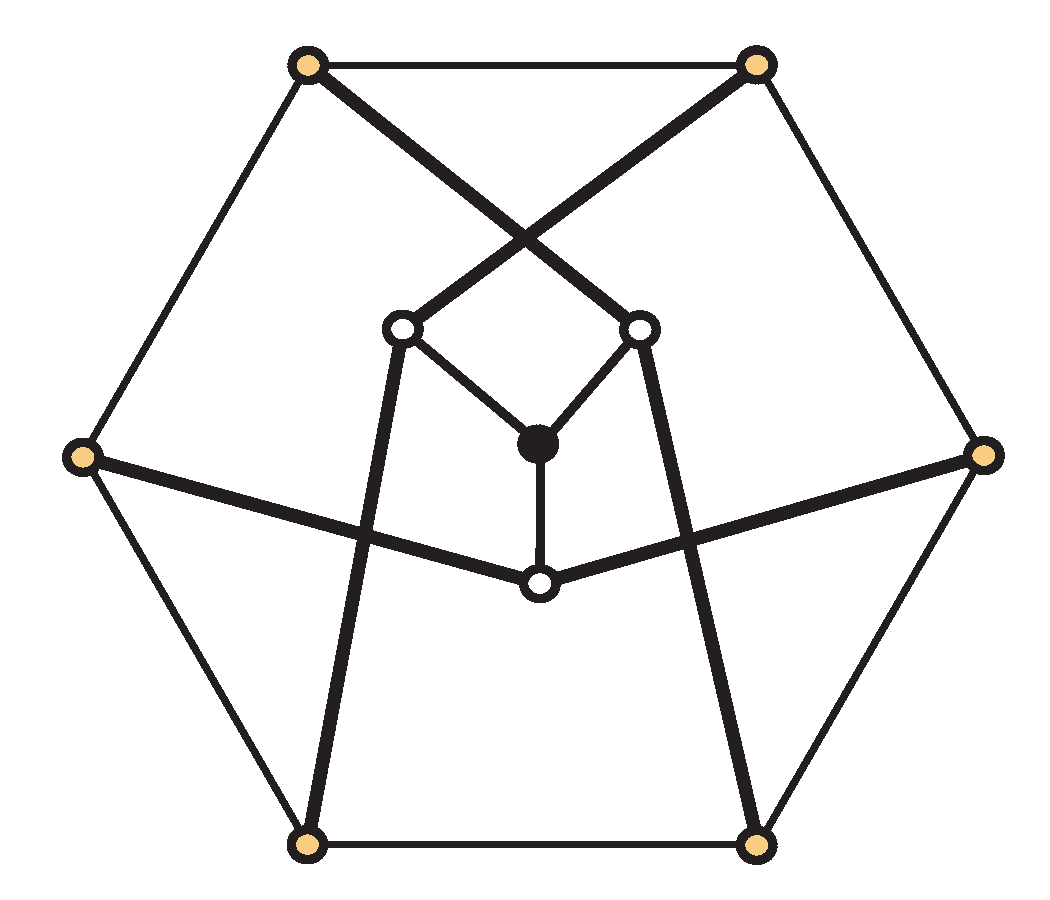
\includegraphics[scale=0.4]{graphs-figs/petersen_graph_k33}
  \caption{A more illustrative drawing of the Petersen graph}
  \label{fig:petersen-graph-k33}
\end{figure}

We close this section with a problem that brings the current section
together with the topic of graph coloring. In 1852 Francis Guthrie, an
Englishman who was at the time studying to be lawyer but subsequently
became a professor of mathematics in South Africa, was trying to color
a map of the counties of England so that any two counties that shared
a boundary segment (meaning they touched in more than a single point)
were colored with different colors. He noticed that he only needed
four colors to do this, and was unable to draw any sort of map that
would require five colors. (He was able to find a map that required
four colors, an example of which is shown in
\autoref{fig:needs-four-colors}.)
\begin{figure}
  \centering
  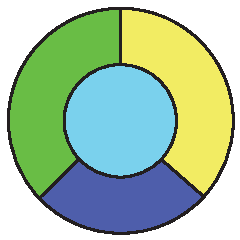
\includegraphics{graphs-figs/needs_four_colors}
  \caption{A map that requires four colors}
  \label{fig:needs-four-colors}
\end{figure}
Could it possibly be true that \emph{every} map could be colored with
only four colors? He asked his brother Frederick Guthrie, who was a
mathematics student at University College, London, about the problem,
and Frederick eventually communicated the problem to Augustus de
Morgan (of de Morgan's laws fame), one of his teachers. It was in this
way that one of the most famous (or infamous) problems, known for a
century as the Four Color Problem and now the Four Color Theorem, in
graph theory was born. De Morgan was very interested in the Four Color
Problem, and communicated it to Sir William Rowan Hamilton,  a
prominent Irish mathematician and the one for whom hamiltonian
cycles are named, but Hamilton did not find the problem
interesting. Hamilton is one of the few people who considered the Four
Color Problem but did not become captivated by it.

We'll continue our discussion of the history of the Four Color Theorem
in a moment, but first, we must consider how we can turn the problem
of coloring a map into a graph theory question. Well, it seems natural
that each region should be assigned a corresponding vertex. We want to
force regions that share a boundary to have different colors, so this
suggests that we should place an edge between two vertices if and only
if their corresponding regions have a common boundary. (As an example,
the map in \autoref{fig:needs-four-colors} corresponds to the graph
$\bfK_4$.) It is not difficult to see that this produces a planar
graph, since we may draw the edges through the common boundary
segment. Furthermore, with a little bit of thought, you should see
that given a planar drawing of a graph, you can create a map in which
each vertex leads to a region and edges lead to common boundary
segments. Thus, the Four Color Problem could be stated as ``Does every
planar graph have chromatic number at most four?''

Interest in the Four Color Problem languished until 1877, when the
British mathematician Arthur Cayley worte a letter to the Royal
Society asking if the problem had been resolved. This brought the
problem to the attention of many more people, and the first ``proof''
of the Four Color Theorem, due to Alfred Bray Kempe, was completed in
1878 and published a year later. It took $11$ years before Percy John
Heawood found a flaw in the proof but was able to salvage enough of it
to show that every planar graph has chromatic number at most five. In
1880, Peter Guthrie Tait, a British physicist best known for his book
\textit{Treatise on Natural Philosophy} with Sir William Thomson (Lord
Kelvin), made an announcement that suggested he had a proof of the
Four Color Theorem utilizing hamiltonian cycles in certain planar
graphs. However, consistent with the way Tait approached some
conjectures in the mathematical theory of knots, it appears that he
subsequently realized around 1883 that he could not prove that the
hamiltonian cycles he was using actually existed and so Tait likely
only believed he had a proof of the Four Color Theorem for a short
time, if at all. However, it would take until 1946 to find a
counterexample to the conjecture Tait had used in his attempt to prove
the Four Color Theorem.

In the first half of the twentieth century, some incremental progress
toward resolving the Four Color Problem was made, but few prominent
mathematicians took a serious interest in it. The final push to prove
the Four Color Theorem came with about at the same time that
the first electronic computers were coming into widespread use in
industry and research. In 1976, two mathematicians at the University
of Illinois announced their computer-assisted proof of the Four Color
Theorem. The proof by Kenneth Appel and Wolfgang Haken led the
University of Illinois to add the phrase ``FOUR COLORS
SUFFICE'' to its postage meter's imprint.\footnote{A photograph of an envelope with such a meter mark
  on it can be found in the book \textit{The Four-Color Theorem:
    History, Topological Foundations, and Idea of Proof} by Rudolf and
  Gerda Fritsch. (Springer, 1998)}

\begin{theorem}[Four Color Theorem]\label{thm:4ct}
  Every planar graph has chromatic number at most four.
\end{theorem}

Appel and Haken's proof of the Four Color Theorem was at a minimum
unsatisfactory for many mathematicians, and to some it simply wasn't a
proof. These mathematicians felt that the using a computer to check
various cases was simply too uncertain; how could you be certain that
the code that checked the 1,482 ``unavoidable configurations'' didn't
contain any logic errors? In fact, there were several mistakes found
in the cases analyzed, but none were found to be fatal flaws. In 1989,
Appel and Haken published a 741-page tome entitled \textit{Every
  Planar Map is Four Colorable} which provided corrections to all
known flaws in their original argument. This still didn't satisfy
many, and in the early 1990's a team consisting of Neil Robertson from
The Ohio State University; Daniel P. Sanders, a graduate student at
the Georgia Institute of Technology; Paul Seymour of
Bellcore; and Robin Thomas from Georgia Tech announced a new proof of
the Four Color Theorem. However, it still required the use of
computers. The proof did gain more widespread acceptance than that of
Appel and Haken, in part because the new proof used fewer than half
($633$) of the number of configurations the Appel-Haken proof used and
the computer code was provided online for anyone to verify. While
still unsatisfactory to many, the proof by Robertson, et al. was
generally accepted, and today the issue of the Four Color Theorem has
largely been put to rest. However, many still wonder if anyone will
ever find a proof of this simple statement that does not require the
assistance of a computer.

\section{Counting Labeled Trees}\label{s:graphs:counting-trees}

How many trees are there with vertex set $[n]=\{1,2,\dots,n\}$? Let
$T_n$ be this number. For $n=1$, there is clearly only one tree. Also,
for $n=2$, there is only one tree, which is isomorphic to $\bfK_2$. In
determining $T_3$, we finally have some work to do; however, there's
not much, since all trees on $3$ vertices are isomorphic to
$\bfP_3$. Thus, there are $T_3=3$ \emph{labeled} trees on $3$
vertices, corresponding to which vertex is the one of degree $2$. When
$n=4$, we can begin by counting the number of nonisomorphic trees and
consider two cases depending on whether the tree has a vertex of
degree $3$.  If there is a vertex of degree $3$, the tree is
isomorphic to $\bfK_{1,3}$ or it does not have a vertex of degree
three, in which case it is isomorphic to $\bfP_4$, since there must be
precisely two vertices of degree $2$ in such a graph. There are four
labelings by $[4]$ for $\bfK_{1,3}$ (choose the vertex of degree
three). How many labelings by $[4]$ are there for $\bfP_4$? There are
$C(4,2)$ ways to choose the labels $i,j$ given to the vertices of
degree $2$ and two ways to select one of the remaining labels to be
made adjacent to $i$. Thus, there are $12$ ways to label $\bfP_4$ by
$[4]$ and so $T_4=16$.

To this point, it looks like maybe there's a pattern forming. Perhaps
it is the case that for all $n\geq 1$, $T_n = n^{n-2}$. This is in
fact the case, but let's see how it works out for $n=5$ before proving
the result in general. What are the nonisomorphic trees on five
vertices? Well, there's $\bfK_{1,4}$ and $\bfP_5$ for sure, and
there's also the third tree shown in \autoref{fig:trees-5verts}. After
thinking for a minute or two, you should be able to convince yourself
that this is all of the possibilities. How many labelings by $[5]$
does each of these have? There are $5$ for $\bfK_{1,4}$ since there
are $5$ ways to choose the vertex of degree $4$. For $\bfP_5$, there
are $5$ ways to choose the middle vertex of the path, $C(4,2)=6$ ways
to label the two remaining vertices of degree $2$ once the middle
vertex is labeled, and then $2$ ways to label the vertices of degree
$1$. This gives $60$ labelings. For the last tree, there are $5$ ways
to label the vertex of degree $3$, $C(4,2)=6$ ways to label the two
leaves adjacent to the vertex of degree $3$, and $2$ ways to label the
remaining two vertices, giving $60$ labelings. Therefore,
$T_5=125=5^3=5^{5-2}$.
\begin{figure}
  \centering
  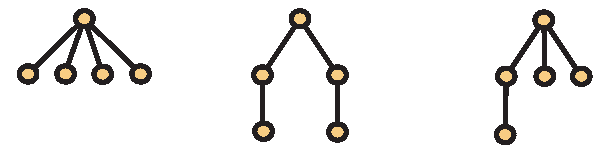
\includegraphics{graphs-figs/trees-5verts}
  \caption{The nonisomorphic trees on $n=5$ vertices}
  \label{fig:trees-5verts}
\end{figure}

It turns out that we are in fact on the right track, and we will now
set out to prove the following:
\begin{theorem}[Cayley's Formula]\label{thm:cayley}
  The number $T_n$ of labeled trees on $n$ vertices is $n^{n-2}$.
\end{theorem}
\noindent This result is usually referred to as Cayley's Formula,
although equivalent results were proven earlier by James J.\ Sylvester
(1857) and Carl W.\ Borchardt (1860). The reason that Cayley's name is
most often affixed to this result is that he was the first to state
and prove it in graph theoretic terminology (in 1889). (Although one
could argue that Cayley really only proved it for $n=6$ and then
claimed that it could easily be extended for all other values of $n$,
and whether such an extension can actually happen is open to some
debate.) Cayley's Formula has many different proofs, most of which are
quite elegant. If you're interested in presentations of several
proofs, we encourage you to read the chapter on Cayley's Formula in
\textit{Proofs from THE BOOK} by Aigner, Ziegler, and Hofmann, which
contains four different proofs, all using different proof
techniques. Here we give a fifth proof, due to Pr\"ufer and published
in 1918. Interestingly, even though Pr\"ufer's proof came after much
of the terminology of graph theory was established, he seemed unaware
of it and worked in the context of permutations and his own
terminology, even though his approach clearly includes the ideas of
graph theory. We will use a recursive technique in order to find a
bijection between the set of labeled trees on $n$ vertices and a
natural set of size $n^{n-2}$, the set of strings of length $n-2$
where the symbols in the string come from $[n]$.

We define a recursive algorithm that takes a tree $\bfT$ on $k\geq 2$
vertices labeled by elements of a set $S$ of positive integers of size
$k$ and returns a string of length $k-2$ whose symbols are elements of
$S$. (The set $S$ will usually be $[k]$, but in order to define a
recursive procedure, we need to allow that it be an arbitrary set of
$k$ positive integers.) This string is called the \textit{Pr\"ufer
  code} of the tree $\bfT$. Let $\prufer(\bfT)$ denote the
Pr\"ufer code of the tree $\bfT$, and if $v$ is a leaf of $\bfT$, let
$\bfT-v$ denote the tree obtained from $\bfT$ by removing $v$ (i.e.,
the subgraph induced by all the other vertices). We can then define
$\prufer(\bfT)$ recursively by
\begin{enumerate}
\item If $\bfT\cong \bfK_2$, return the empty string.
\item Else, let $v$ be the leaf of $\bfT$ with the smallest label
  and let $u$ be its unique neighbor. Let $i$ be the label of
  $u$. Return $(i,\prufer(\bfT-v))$.
\end{enumerate}

\begin{example}\label{ex:prufer-code}
  Before using Pr\"ufer codes to prove Cayley's Formula, let's take a
  moment to make sure we understand how they are computed given a
  tree. Consider the $9$-vertex tree $\bfT$ in \autoref{fig:prufer-code}.
  \begin{figure}[h]
    \centering
    \begin{overpic}{graphs-figs/tree-9verts}
      \put(46,2){$1$}
      \put(21,21){$2$}
      \put(62,14.5){$3$}
      \put(36.8,14.5){$4$}
      \put(2,2){$5$}
      \put(9,12){$6$}
      \put(90,12){$7$}
      \put(27.5,5.5){$8$}
      \put(77.3,21){$9$}
    \end{overpic}
    \caption{A labeled $9$-vertex tree}
    \label{fig:prufer-code}
  \end{figure}
How do we compute $\prufer(\bfT)$? Since $\bfT$ has more than two
vertices, we use the second step and find that $v$ is the vertex with
label $2$ and $u$ is the vertex with label $6$, so
$\prufer(\bfT)=(6,\prufer(\bfT-v))$. The graph $\bfT-v$ is
shown in \autoref{fig:prufer-code-delete1}.
  \begin{figure}[h]
    \centering
    \begin{overpic}{graphs-figs/tree-8verts}
      \put(46,2){$1$}
%      \put(21,21){$2$}
      \put(62,14.5){$3$}
      \put(36.8,14.5){$4$}
      \put(2,2){$5$}
      \put(9,12){$6$}
      \put(90,12){$7$}
      \put(27.5,5.5){$8$}
      \put(77.3,21){$9$}
    \end{overpic}
    \caption{The tree $\bfT-v$}
    \label{fig:prufer-code-delete1}
  \end{figure}
  The recursive call $\prufer(\bfT-v)$ returns
  $(6,\prufer(\bfT-v-v'))$, where $v'$ is the vertex labeled
  $5$. Continuing recursively, the next vertex deleted is $6$, which
  appends a $4$ to the string. Then $7$ is deleted, appending
  $3$. Next $8$ is deleted, appending $1$. This is followed by the
  deletion of $1$, appending $4$. Finally $4$ is deleted, appending
  $3$, and the final recursive call has the subtree isomorphic to
  $\bfK_2$ with vertices labeled $3$ and $9$, and an empty string is
  returned. Thus, $\prufer(\bfT)=6643143$.
\end{example}

We're now prepared to give a proof of Cayley's Formula.

\begin{proof}
  It is clear that $\prufer(\bfT)$ takes an $n$-vertex labeled tree
  with labels from $[n]$ and returns a string of length $n-2$ whose
  symbols are elements of $[n]$. What we have yet to do is determine a
  way to take such a string and construct an $n$-vertex labeled tree
  from it. If we can find such a construction, we will have a
  bijection between the set $\mathcal{T}_n$ of labeled trees on $n$
  vertices and the set of strings of length $n-2$ whose symbols come
  from $[n]$, which will imply that $T_n=n^{n-2}$.

  First, let's look at how $\prufer(\bfT)$ behaves. What numbers
  actually appear in the Pr\"ufer code? The numbers that appear in the
  Pr\"ufer code are the labels of the \textit{nonleaf} vertices of
  $\bfT$. The label of a leaf simply cannot appear, since we always
  record the label of the \textit{neighbor} of the leaf we are
  deleting, and the only way we would delete the neighbor of a leaf is
  if that neighbor were also a leaf, which can only happen
  $\bfT\cong\bfK_2$, in which case $\prufer(\bfT)$ simply returns the
  empty string. Thus if $I\subset [n]$ is the set of symbols that
  appear in $\prufer(\bfT)$, the labels of the leaves of $\bfT$ are
  precisely the elements of $[n]-I$.

  With the knowledge of which labels belong to the leaves of $\bfT$ in
  hand, we are ready to use induction to complete the proof. Our goal
  is to show that if given a string $\bfs=s_1s_2\cdots s_{n-2}$ whose
  symbols come from a set $S$ of $n$ elements, there is a unique tree
  $\bfT$ with $\prufer(\bfT) = \bfs$. If $n=2$, the only such string
  is the empty string, so $1$ and $2$ both label leaves and we can
  construct only $\bfK_2$. Now suppose we have the result for some
  $m\geq 2$, and we try to prove it for $m+1$. We have a string $\bfs
  = s_1s_2\cdots s_{m-1}$ with symbols from $[m+1]$. Let $I$ be the
  set of symbols appearing in $\bfs$ and let $k$ be the least element
  of $[m+1]-I$. By the previous paragraph, we know that $k$ is the
  label of a leaf of $\bfT$ and that is unique neighbor is the vertex
  labeled $s_1$. The string $\bfs'=s_2s_3\cdots s_{m-1}$ has length
  $m-2$ and since $k$ does not appear in $\bfs$, its symbols come from
  $S=[m+1]-\{k\}$, which has size $m$. Thus, by induction, there is a
  unique tree $\bfT'$ whose Pr\"ufer code is $\bfs'$. We form $\bfT$
  from $\bfT'$ by attaching a leaf with label $k$ to the vertex of
  $\bfT'$ with label $s_1$ and have a tree of the desired type.
\end{proof}

\begin{example}\label{ex:prufer-code-reverse}
  We close this section with an example of how to take a Pr\"ufer code
  and use it to construct a labeled tree. Consider the string
  $\bfs=75531$ as a Pr\"ufer code. Then the tree $\bfT$ corresponding
  to $\bfs$ has $7$ vertices, and its leaves are labeled $2$, $4$, and
  $6$. The inductive step in our proof attaches the vertex labeled $2$
  to the vertex labeled $7$ in the tree $\bfT'$ with Pr\"ufer code
  $5531$ and vertex labels $\{1,3,4,5,6,7\}$, since $2$ is used to
  label the last vertex added. What are the leaves of $\bfT'$? The
  symbols in $\{4,6,7\}$ do not appear in $5531$, so they must be the
  labels of leaves, and the construction says that we would attach the
  vertex labeled $4$ to the vertex labeled $5$ in the tree we get by
  induction. In \autoref{tab:prufer-code-reverse}, we show how this
  recursive process continues.
  \begin{table}[h]
    \centering
    \begin{tabular}{ccc}
      Pr\"ufer code & Label set & Edge added\\
      75531 & $\{1,2,3,4,5,6,7\}$ & 2--7\\
      5531 & $\{1,3,4,5,6,7\}$ & 4--5\\
      531 & $\{1,3,5,6,7\}$ & 6--5\\
      31 & $\{1,3,5,7\}$ & 5--3\\
      1 & $\{1,3,7\}$ & 3--1\\
      (empty string) & $\{1,7\}$ & 1--7
    \end{tabular}
    \caption{Turning the Pr\"ufer code $75531$ into a labeled tree}
    \label{tab:prufer-code-reverse}
  \end{table}
  We form each row from the row above it by removing the first label
  used on the edge added from the label set and removing the first
  symbol from the Pr\"ufer code. Once the Pr\"ufer code becomes the
  empty string, we know that the two remaining labels must be the
  labels we place on the ends of $\bfK_2$ to start building $\bfT$. We
  then work back up the edge added column, adding a new vertex and the
  edge indicated. The tree we construct in this manner is shown in
  \autoref{fig:prufer-code-reverse}.
  \begin{figure}[h]
    \centering
    \begin{overpic}{graphs-figs/prufer-code-reverse}
      \put(2,21){$4$}
%      \put(21,21){$2$}
      \put(62,14.5){$1$}
      \put(36.8,14.5){$3$}
      \put(2,2){$6$}
      \put(9,12){$5$}
      \put(90,12){$7$}
      \put(93,21){$2$}
    \end{overpic}
    \caption{The labeled tree with Pr\"ufer code $75531$}
    \label{fig:prufer-code-reverse}
  \end{figure}
\end{example}

%\section{Matchings in Graphs}\label{s:graphs:matching}

%This space reserved for a future section focusing on Hall's theorem
%but also talking about general matchings.

\section{A Digression into Complexity Theory}\label{s:graphs:complexity}

We have already introduced in \autoref{ch:basics} a few notions about
efficient algorithms. We also discussed the difficulty of determining
a graph's chromatic number and clique number earlier in this
chapter. We conclude with a brief discussion of some issues involving
computational complexity for other problems discussed in this chapter.

Let's begin with some problems for which there are polynomial-time
algorithms. Suppose you are given a graph on $n$ vertices and asked
whether or not the graph is connected. Here a positive answer can be
justified by providing a spanning tree.  On the other hand, a negative
answer can be justified by providing a partition of the vertex sets
$V=V_1\cup V_2$ with $V_1$ and $V_2$ non-empty subsets and having no
edges with one end-point in $V_1$ and the other in $V_2$. In
\autoref{ch:graphalgorithms} we will discuss two efficient algorithms
that find spanning trees in connected graphs. They can easily be
modified to produce a partition showing the graph is disconnected.

If you are asked whether a connected graph is eulerian, then a
positive answer can be justified by producing the appropriate
sequence. We gave an algorithm to do this earlier in the chapter. A
negative answer can be justified by producing a vertex of odd degree,
and our algorithm will identify such a vertex if it exists. (Depending
on the data structures used to represent the graph, it may be most
efficient to simply look for vertices of odd degree without using the
algorithm to find an eulerian circuit.)

On the surface, the problem of determining if a graph is hamiltonian
looks similar to that of determining if the graph is eulerian. Both
call for a sequence of vertices in which each pair of consecutive
vertices is joined by an edge. Of course, each problem has an
additional requirement on yes certificates. However, justifying a
negative answer to the question of whether a graph is hamiltonian is
not straightforward. \autoref{thm:graphs:dirac} only gives a way to
confirm that a graph \emph{is} hamiltonian; there are many
nonhamiltonian graphs that do not satisfy its hypothesis. At this
time, no one knows how to justify a negative answer---at least not in
the general case.

\section{Discussion}

Over coffee, today's conversation was enthusiastic and heated at
times. Zori got things off with a blast ``I don't think graphs
are of any use at all\dots'' but she wasn't even able to finish
the sentence before Yolanda  uncharacteristically interrupted her with
``You're off base on this one.  I see lots of ways graphs can
be used to model real world problems.  The professor actually
showed us examples back in our first class.  But now that we're
talking in more depth about graphs, things are even clearer.''
Bob added ``These eulerian and hamiltonian cycle problems are
certain to have applications in network routing problems.''
Xing reinforced Bob with ``Absolutely.  There are important
questions in network integrity and information exchange that
are very much the same as these basic problems.'' Alice piled
on ``Even the notion of chromatic number clearly has practical
applications.''  By this time, Zori realized her position was
indefensible but she was reluctant to admit it.  She offered
only a ``Whatever.''

Things quieted down a bit and Dave said ``Finding a hamiltonian
cycle can't be all that hard, if someone guarantees that there
is one.  This extra information must be of value in the search.''
Xing added ``Maybe so.  It seems natural that it should be
easier to find something if you know it's there.''  Alice
asked ``Does the same thing hold for chromatic number?''  Bob
didn't understand her question ``Huh?''  Alice continued,
this time being careful not to even look Bob's way ``I mean
if someone tells you that a graph is $3$-colorable, does that
help you to find a coloring using only three colors?''  Dave
said ``Seems reasonable to me.''

After a brief pause, Carlos offered ``I don't think this extra
knowledge is of any help. I think these problems are pretty hard,
regardless.''  They went back and forth for a while, but in the
end, the only thing that was completely clear is that graphs
and their properties had captured their attention, at least for
now.

\section{Exercises}\label{s:graphs:exercises}
\begin{enumerate}
\item The questions in this exercise pertain to the graph $\bfG$ shown in
  \autoref{fig:graphs:graph_ex}.
  \begin{enumerate}
  \item What is the degree of vertex $8$?
  \item What is the degree of vertex $10$?
  \item How many vertices of degree $2$ are there in $\bfG$? List
    them.
  \item Find a cycle of length $8$ in $\bfG$.
  \item What is the length of a shortest path from $3$ to $4$?
  \item What is the length of a shortest path from $8$ to $7$?
  \item Find a path of length $5$ from vertex $4$ to vertex $6$.
  \end{enumerate}
 \begin{figure}[h]
    \centering
    \includegraphics*[height=1.75in]{graphs-figs/graph_ex}    
    \caption{A graph}
    \label{fig:graphs:graph_ex}
  \end{figure}
\item Draw a graph with $8$ vertices, all of odd degree, that does not
  contain a path of length $3$ or explain why such a graph does not
  exist.
\item Draw a graph with $6$ vertices having degrees $5$, $4$, $4$,
  $2$, $1$, and $1$ or explain why such a graph does not exist.
\item For the next Olympic Winter Games, the organizers wish to expand
  the number of teams competing in curling. They wish to have $14$
  teams enter, divided into two pools of seven teams each. Right now,
  they're thinking of requiring that in preliminary play each team
  will play seven games against distinct opponents. Five of the
  opponents will come from their own pool and two of the opponents
  will come from the other pool. They're having trouble setting up
  such a schedule, so they've come to you. By using an appropriate
  graph-theoretic model, either argue that they cannot use their
  current plan or devise a way for them to do so.
\item For this exercise, consider the graph $\bfG$ in
  \autoref{fig:graphs:subgraphs_ex}.
  \begin{enumerate}
  \item Let $V_1=\{g,j,c,h,e,f\}$ and $E_1=\{ge,jg,ch,ef\}$. Is
    $(V_1,E_1)$ a subgraph of $\bfG$?
  \item Let $V_2=\{g,j,c,h,e,f\}$ and $E_2=\{ge,jg,ch,ef,cj\}$. Is
    $(V_2,E_2)$ a subgraph of $\bfG$?
  \item Let $V_3=\{a,d,c,h,b\}$ and $E_3=\{ch,ac,ad,bc\}$. Is
    $(V_3,E_3)$ an induced subgraph of $\bfG$?
  \item Draw the subgraph of $\bfG$ induced by $\{g,j,d,a,c,i\}$.
  \item Draw the subgraph of $\bfG$ induced by $\{c,h,f,i,j\}$.
  \item Draw a subgraph of $\bfG$ having vertex set $\{e,f,b,c,h,j\}$
    that is \emph{not} an induced subgraph.
  \item Draw a spanning subgraph of $\bfG$ with exactly $10$ edges.
  \end{enumerate}
 \begin{figure}[h]
    \centering
    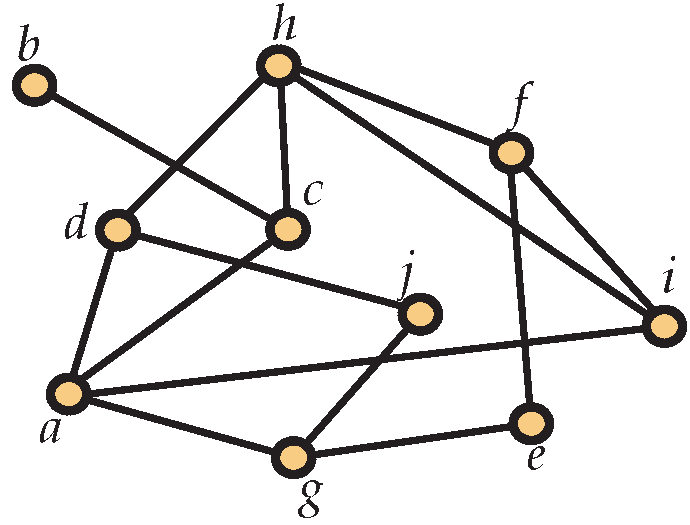
\includegraphics[scale=0.5]{graphs-figs/subgraphs_ex}
    \caption{A graph $\bfG$}
    \label{fig:graphs:subgraphs_ex}
  \end{figure}
\item Prove that every tree on $n$ vertices has exactly $n-1$ edges.
\item \autoref{fig:graphs:isomorphic_ex} contains four graphs on six
  vertices. Determine which (if any) pairs of graphs are
  isomorphic. For pairs that are isomorphic, give an isomorphism
  between the two graphs. For pairs that are not isomorphic, explain
  why.
  \begin{figure}[h]
    \centering
    \begin{overpic}[scale=0.6]{graphs-figs/isomorphic_ex}
      \put(22,47){$\bfG_1$}
      \put(74,47){$\bfG_2$}
      \put(22,-5){$\bfG_3$}
      \put(74,-5){$\bfG_4$}
      \put(4,87){$v_1$} \put(22,87){$v_2$} \put(41,87){$v_3$}
      \put(4,54){$v_4$} \put(22,54){$v_5$} \put(41,54){$v_6$}
      \put(63,96){$u_1$} \put(84,96){$u_2$} \put(99,73){$u_3$}
      \put(89,55){$u_4$} \put(57,55){$u_5$} \put(46.5,73){$u_6$}
      \put(10,41){$w_1$} \put(31.5,41){$w_2$} \put(45.5,20){$w_3$}
      \put(37,3){$w_4$} \put(3,3){$w_5$} \put(-7.5,21){$w_6$}
      \put(56,38.3){$x_1$} \put(74,38.3){$x_2$} \put(92,38.3){$x_3$}
      \put(56,5){$x_4$} \put(74,5){$x_5$} \put(92,5){$x_6$}
    \end{overpic}
    \caption{Are these graphs isomorphic?}
    \label{fig:graphs:isomorphic_ex}
  \end{figure}
\item Find an eulerian circuit in the graph $\bfG$ in
  \autoref{fig:graphs:euler_exercise} or explain why one does not
  exist.
  \begin{figure}[h]
    \begin{center}
      \begin{overpic}[width=4in]{graphs-figs/euler_exercise}
        \put(6,19.5){$1$}
        \put(64.3,5){$2$}
        \put(43.8,15){$3$}
        \put(60,23.5){$4$}
        \put(26,2){$5$}
        \put(21,32){$6$}
        \put(85,9){$$7}
        \put(32.3,26.3){$8$}
        \put(53,-1){$9$}
        \put(42,33){$10$}
        \put(71,26){$11$}
        \put(83,21){$12$}
      \end{overpic}
      \caption{A graph $\bfG$}\label{fig:graphs:euler_exercise}
    \end{center}
  \end{figure}
\item Consider the graph $\bfG$ in \autoref{fig:graphs:euler_hamilton_ex}. Determine if the graph is eulerian. If
  it is, find an eulerian circuit. If it is not, explain why it is
  not. Determine if the graph is hamiltonian. If it is, find a
  hamiltonian cycle. If it is not, explain why it is not.
  \begin{figure}
  \begin{center}
    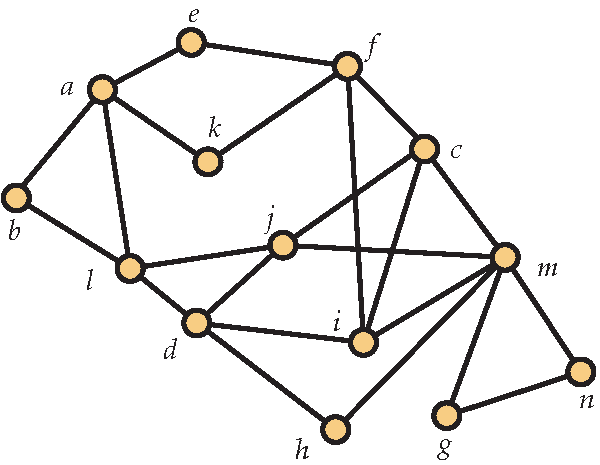
\includegraphics[width=2.5in]{graphs-figs/euler_hamilton_ex}
    \caption{A graph $\bfG$}\label{fig:graphs:euler_hamilton_ex}
 \end{center}
 \end{figure}
\item Explain why the graph $\bfG$ in
  \autoref{fig:graphs:noneuler_exercise} does not have an eulerian
  circuit, but show that by adding a single edge, you can make it
  eulerian.
  \begin{figure}[h]
    \begin{center}
      \begin{overpic}[width=4in]{graphs-figs/noneuler_exercise}
        \put(6,19.5){$1$}
        \put(67,3){$2$}
        \put(48,11){$3$}
        \put(64,33){$4$}
        \put(3,4){$5$}
        \put(21,26){$6$}
        \put(85,9){$$7}
        \put(24.7,12.8){$8$}
        \put(45,-1){$9$}
        \put(32,35){$10$}
        \put(72,24){$11$}
        \put(61,10){$12$}
      \end{overpic}
      \caption{A graph $\bfG$}\label{fig:graphs:noneuler_exercise}
    \end{center}
  \end{figure}
\item An \emph{eulerian trail} is defined in the same manner as an
  euler circuit (see
  \hyperref[def:eulerian-circuit]{page~\pageref*{def:eulerian-circuit}})
  except that we drop the condition that $x_0=x_t$. Prove that a
  graph has an eulerian trail if and only if it is connected and has
  at most two vertices of odd degree.
\item Alice and Bob are discussing a graph that has $17$ vertices and
  $129$ edges. Bob argues that the graph is Hamiltonian, while Alice
  says that he's wrong. Without knowing anything more about the graph,
  must one of them be right? If so, who and why, and if not, why not?
\item Find the chromatic number of the graph $\bfG$ in
  \autoref{fig:graphs:bipartite_ex} and a coloring using $\chi(\bfG)$ colors.
  \begin{figure}[h]
    \centering
    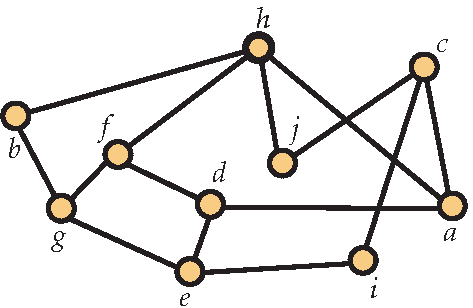
\includegraphics[scale=0.6]{graphs-figs/bipartite_ex}
    \caption{A graph $\bfG$ to color}
    \label{fig:graphs:bipartite_ex}
  \end{figure}
\item Find the chromatic number of the graph $\bfG$ in
  \autoref{fig:graphs:coloring_ex} and a coloring using $\chi(\bfG)$ colors.
  \begin{figure}[h]
    \centering
    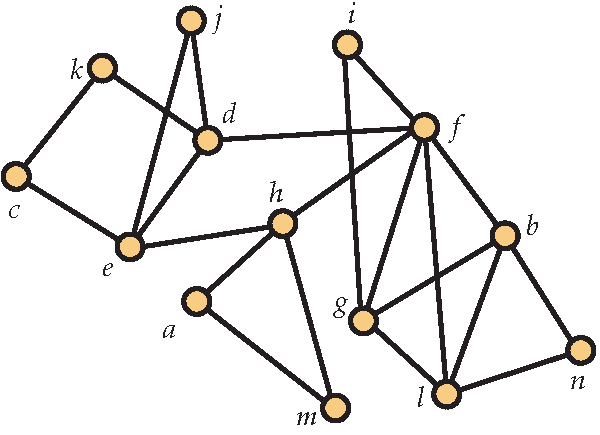
\includegraphics[scale=0.6]{graphs-figs/coloring_ex}
    \caption{A graph $\bfG$ to color}
    \label{fig:graphs:coloring_ex}
  \end{figure}
\item A pharmaceutical manufacturer is building a new warehouse to
  store its supply of $10$ chemicals it uses in production. However,
  some of the chemicals cannot be stored in the same room due to undesirable
  reactions that will occur. The matrix below has a $1$ in position
  $(i,j)$ if and only if chemical $i$ and chemical $j$ cannot be
  stored in the same room. Develop an appropriate graph theoretic
  model and determine the smallest number of rooms into which they can
  divide their warehouse so that they can safely store all $10$
  chemicals in the warehouse.
  \[
  \begin{bmatrix}
    0 & 1 & 0 & 1 & 1 & 0 & 1 & 0 & 0 & 0\\
    1 & 0 & 0 & 1 & 1 & 0 & 0 & 0 & 0 & 1\\
    0 & 0 & 0 & 0 & 0 & 1 & 0 & 1 & 1 & 0\\
    1 & 1 & 0 & 0 & 1 & 0 & 0 & 0 & 0 & 0\\
    1 & 1 & 0 & 1 & 0 & 0 & 0 & 0 & 1 & 0\\
    0 & 0 & 1 & 0 & 0 & 0 & 1 & 0 & 0 & 1\\
    1 & 0 & 0 & 0 & 0 & 1 & 0 & 1 & 0 & 0\\
    0 & 0 & 1 & 0 & 0 & 0 & 1 & 0 & 0 & 0\\
    0 & 0 & 1 & 0 & 1 & 0 & 0 & 0 & 0 & 0\\
    0 & 1 & 0 & 0 & 0 & 1 & 0 & 0 & 0 & 0
  \end{bmatrix}
  \]
\item A school is preparing the schedule of classes for the next
  academic year. They are concerned about scheduling calculus,
  physics, English, statistics, economics, chemistry, and German
  classes, planning to offer a single section of each one. Below are
  the lists of courses that each of six students must take in order to
  successfully graduate. Determine the smallest number of class
  periods that can be used to schedule these courses if each student
  can take at most one course per class period. Explain why fewer
  class periods cannot be used.
  \begin{center}
    \begin{tabular}{c|l}
      Student & Courses\\\hline
      1 & Chemistry, Physics, Economics\\
      2 & English, German, Statistics\\
      3 & Statistics, Calculus, German\\
      4 & Chemistry, Physics\\
      5 & English, Chemistry\\
      6 & Chemistry, Economics
    \end{tabular}
  \end{center}
\item All trees with more than one vertex have the same chromatic
  number. What is it, and why?
\item \label{ex:color} Find a proper $(t+1)$-coloring of the
  graph $\bfG_{t+1}$ in Mycielski's proof of
  \hyperref[prop:triangle-free]{Proposition~\ref*{prop:triangle-free}}. This
  establishes that $\chi(\bfG_{t+1})\leq t+1$.
\item How many vertices does the graph $\bfG_4$ from the Kelly and
  Kelly proof of
  \hyperref[prop:triangle-free]{Proposition~\ref*{prop:triangle-free}}
  have?
\item Construct and draw the graph $\bfG_5$ from Mycielski's proof of
  \hyperref[prop:triangle-free]{Proposition~\ref*{prop:triangle-free}}.
\item Find a recursive formula for the number of vertices $n_t$ in the
  graph $\bfG_t$ from the Kelly and Kelly proof of
  \hyperref[prop:triangle-free]{Proposition~\ref*{prop:triangle-free}}.
\item Let $b_t$ be the number of vertices in the graph $\bfG_t$ from
  the Mycielski's proof of
  \hyperref[prop:triangle-free]{Proposition~\ref*{prop:triangle-free}}. Find
  a recursive formula for $b_t$.
\item The \emph{girth} of a graph $\bfG$ is the number of vertices in
  a shortest cycle of $\bfG$. Find the girth of the graph $\bfG_t$ in
  the Kelly and Kelly proof of
  \hyperref[prop:triangle-free]{Proposition~\ref*{prop:triangle-free}}
  and prove that your answer is correct. As a challenge, see if you
  can modify the construction of $\bfG_t$ to increase the girth. If
  so, how far are you able to increase it?
\item \label{ex:graphs:first-fit-color}Use the First Fit algorithm to
  color the graph in \autoref{fig:k44minus} using the two different
  orderings of the vertex set shown there.
\item Draw the interval graph corresponding to the intervals in
  \autoref{fig:graphs:intervals-ex}.
  \begin{figure}[h]
    \centering
    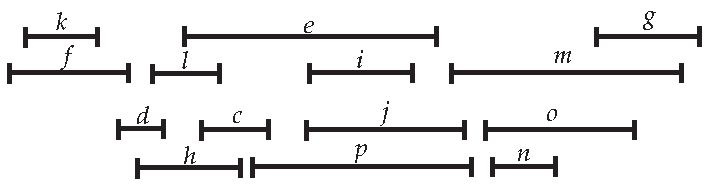
\includegraphics{graphs-figs/firstfit-intgraph}
    \caption{A collection of intervals}
    \label{fig:graphs:intervals-ex}
  \end{figure}
\item Use the First Fit coloring algorithm to find the chromatic
  number of the interval graph whose interval representation is shown
  in \autoref{fig:graphs:intervals-ex} as well as a proper coloring
  using as few colors as possible.
\item 
  \begin{enumerate}
   \item From
    \hyperref[ex:graphs:first-fit-color]{exercise~\ref*{ex:graphs:first-fit-color}}
    you know that choosing a bad ordering of the vertices of a graph
    can lead to the First Fit coloring algorithm producing a coloring
    that is far from optimal. However, you can use this algorithm to
    prove a bound on the chromatic number. Show that if every vertex
    of $\bfG$ has degree at most $D$, then $\chi(\bfG)\leq D+1$.
  \item Give an example of a bipartite graph with $D=1000$ to show
    that this bound need not be tight.
  \end{enumerate}
\item Is the graph in \autoref{fig:graphs:coloring_ex} planar? If it
  is, find a drawing without edges crossings. If it is not give a reason why it is
  not.
\item Is the graph in \autoref{fig:graphs:planar_ex} planar? If it
  is, find a drawing without edge crossings. If it is not give a reason why it is
  not.
  \begin{figure}[h]
    \centering
    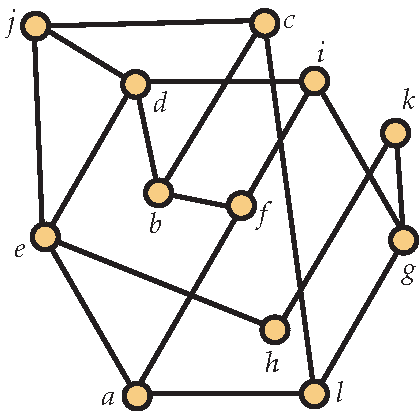
\includegraphics[scale=0.6]{graphs-figs/planar_ex}
    \caption{Is this graph planar?}
    \label{fig:graphs:planar_ex}
  \end{figure}

\item Find a planar drawing of the graph $\bfK_5-e$, by which we mean
  the graph formed from the complete graph on $5$ vertices by deleting
  any edge.
\item Draw a planar drawing of an eulerian planar graph with $10$
  vertices and $21$ edges.
\item Show that every planar graph has a vertex that is incident to at
  most five edges.
\item \label{ex:graphs:degseq}Let $\GVE$ be a graph with $V=\{v_1,v_2,\dots,v_n\}$. Its
  \emph{degree sequence} is the list of the degrees of its vertices,
  arranged in nonincreasing order. That is, the degree sequence of
  $\mathbf{G}$ is
  $(\deg_\mathbf{G}(v_1),\deg_\mathbf{G}(v_2),\dots,\deg_\mathbf{G}(v_n))$
  with the vertices arranged such that $\deg_\mathbf{G}(v_1) \geq
  \deg_\mathbf{G}(v_2)\geq \cdots\geq \deg_\mathbf{G}(v_n)$. Below
  are five sequences of integers (along with $n$, the number of
  integers in the sequence). Identify
  \begin{itemize}
  \item the \textit{one} sequence that \textbf{cannot be the degree
      sequence of any graph};
  \item the \textit{two} sequences that could be the degree sequence
    of a \textbf{planar} graph;
  \item the \textit{one} sequence that could be the degree sequence of
    a \textbf{tree};
  \item the \textit{one} sequence that is the degree sequence of
    an \textbf{eulerian} graph; and
  \item the \textit{one} sequence that is the degree sequence of a
    graph that must be \textbf{hamiltonian}.
  \end{itemize}
  Explain your answers. (Note that one sequence will get two labels
  from above.)
  \begin{enumerate}
  \item $n=10$: $(4,4,2,2,1,1,1,1,1,1)$
  \item $n=9$: $(8,8,8,6,4,4,4,4,4)$
  \item $n=7$: $(5,4,4,3,2,1,0)$
  \item $n=10$: $(7,7,6,6,6,6,5,5,5,5)$
  \item $n=6$: $(5,4,3,2,2,2)$
  \end{enumerate}
\item \label{ex:graphs:degseq2} Below are three sequences of length $10$. One of the sequences
  cannot be the degree sequence (see
  \hyperref[ex:graphs:degseq]{exercise~\ref*{ex:graphs:degseq}}) of
  any graph. Identify it and say why. For each of the other two, say
  \emph{why} (if you have enough information) a \emph{connected} graph
  with that degree sequence
  \begin{itemize}
  \item is definitely hamiltonian/cannot be hamiltonian;
  \item is definitely eulerian/cannot be eulerian;
  \item is definitely a tree/cannot be a tree; and
  \item is definitely planar/cannot be planar.
  \end{itemize}
  (If you do not have enough information to make a determination for a
  sequence without having specific graph(s) with that degree sequence,
  write ``not enough information'' for that property.) 
  \begin{enumerate}
  \item $(6,6,4,4,4,4,2,2,2,2)$
  \item $(7,7,7,7,6,6,6,2,1,1)$
  \item $(8,6,4,4,4,3,2,2,1,1)$
  \end{enumerate}
\item For the two degree sequences in
  \hyperref[ex:graphs:degseq2]{exercise~\ref*{ex:graphs:degseq2}} that
  correspond to graphs, there were some properties for which the
  degree sequence was not sufficient information to determine if the
  graph had that property. For each of those situations, see if you
  can draw both a graph that has the property and a graph that does
  not have the property.
\item Draw the $16$ labeled trees on $4$ vertices.
\item Determine $\prufer(\bfT)$ for the tree $\bfT$ in \autoref{fig:graphs:tree-10verts-ex1}.
  \begin{figure}[h]
    \begin{center}
      \begin{overpic}{graphs-figs/tree-10verts-ex1}
        \put(35,11.2){$1$}
        \put(46,2){$2$}
        \put(22,25){$3$}
        \put(22,9){$4$}
        \put(68,2.5){$5$}
        \put(90,11){$6$}
        \put(5,16){$7$}
        \put(77,21){$8$}
        \put(62,14.5){$9$}
        \put(0.5,2){$10$}
      \end{overpic}
      \caption{A $10$-vertex tree}\label{fig:graphs:tree-10verts-ex1}
    \end{center}
  \end{figure}
\item Determine $\prufer(\bfT)$ for the tree $\bfT$ in \autoref{fig:graphs:tree-10verts-ex2}.
  \begin{figure}[h]
    \begin{center}
      \begin{overpic}{graphs-figs/tree-8verts-ex2}
        \put(50,32){$1$}
        \put(44,2){$2$}
        \put(26,22){$3$}
        \put(31,48){$4$}
        \put(62,56){$5$}
        \put(94,32){$6$}
        \put(5,16){$7$}
        \put(77,21){$8$}
      \end{overpic}
      \caption{A $10$-vertex tree}\label{fig:graphs:tree-10verts-ex2}
    \end{center}
  \end{figure}
\item Determine $\prufer(\bfT)$ for the tree $\bfT$ \autoref{fig:graphs:tree-14verts-ex3}.
  \begin{figure}[h]
    \begin{center}
      \begin{overpic}{graphs-figs/tree-14verts-ex3}
        \put(50,32){$1$}
        \put(44,2){$2$}
        \put(2,34){$3$}
        \put(31,48){$4$}
        \put(62,56){$5$}
        \put(77,21){$6$}
        \put(17,51){$7$}
        \put(94,32){$8$}
        \put(34,20){$9$}
        \put(5,16){$10$}
        \put(74,2){$11$}
        \put(44,9){$12$}
        \put(87,14){$13$}
        \put(64,14){$14$}
    \end{overpic}
    \caption{A $14$-vertex tree}\label{fig:graphs:tree-14verts-ex3}
  \end{center}
\end{figure}
\item Construct the labeled tree $\bfT$ with Pr\"ufer code $96113473$.
\item Construct the labeled tree $\bfT$ with Pr\"ufer code $23134$.
\item Construct the labeled tree $\bfT$ with Pr\"ufer code (using
  commas to separate symbols in the string, since we have labels
  greater than $9$) $10,1,7,4,3,4,10,2,2,8$.
\item (Challenge problem) When $\GVE$ is a graph, let $\Delta(\bfG)$ denote the maximum
  degree in $\bfG$.  Prove \textbf{Brooks' Theorem}:  If $\bfG$ is connected and
  $\Delta(\bfG)=k$, then
  $\chi(\bfG)\le k+1$.  Furthermore, equality holds if and only if
  (a)~$k=2$ and $\bfG$ is an odd cycle, or (b)~$k\neq2$ and $\bfG=\bfK_{k+1}$.
  Hint: It's clear that $\chi(\bfG)\le k+1$ (in fact, this was
  already assigned as an exercise). Assume that $\chi(\bfG)=k+1$
  but that neither conclusion (a) or (b) holds.  Take a spanning tree of
  $\bfG$ and an appropriate ordering of the
  vertices, with two leaves of the tree coming first.  Then show that a 
  First Fit coloring of the graph will only use $k$ colors.
\end{enumerate}


%%% Local Variables: 
%%% mode: latex
%%% TeX-master: "chap-skel-mtk"
%%% End: 
